\documentclass[]{book}
\usepackage{lmodern}
\usepackage{amssymb,amsmath}
\usepackage{ifxetex,ifluatex}
\usepackage{fixltx2e} % provides \textsubscript
\ifnum 0\ifxetex 1\fi\ifluatex 1\fi=0 % if pdftex
  \usepackage[T1]{fontenc}
  \usepackage[utf8]{inputenc}
\else % if luatex or xelatex
  \ifxetex
    \usepackage{mathspec}
  \else
    \usepackage{fontspec}
  \fi
  \defaultfontfeatures{Ligatures=TeX,Scale=MatchLowercase}
\fi
% use upquote if available, for straight quotes in verbatim environments
\IfFileExists{upquote.sty}{\usepackage{upquote}}{}
% use microtype if available
\IfFileExists{microtype.sty}{%
\usepackage{microtype}
\UseMicrotypeSet[protrusion]{basicmath} % disable protrusion for tt fonts
}{}
\usepackage[margin=1in]{geometry}
\usepackage{hyperref}
\hypersetup{unicode=true,
            pdftitle={Government Uncertainty Guidance},
            pdfauthor={Cross-Government Analyst Group},
            pdfborder={0 0 0},
            breaklinks=true}
\urlstyle{same}  % don't use monospace font for urls
\usepackage{natbib}
\bibliographystyle{apalike}
\usepackage{color}
\usepackage{fancyvrb}
\newcommand{\VerbBar}{|}
\newcommand{\VERB}{\Verb[commandchars=\\\{\}]}
\DefineVerbatimEnvironment{Highlighting}{Verbatim}{commandchars=\\\{\}}
% Add ',fontsize=\small' for more characters per line
\usepackage{framed}
\definecolor{shadecolor}{RGB}{248,248,248}
\newenvironment{Shaded}{\begin{snugshade}}{\end{snugshade}}
\newcommand{\KeywordTok}[1]{\textcolor[rgb]{0.13,0.29,0.53}{\textbf{#1}}}
\newcommand{\DataTypeTok}[1]{\textcolor[rgb]{0.13,0.29,0.53}{#1}}
\newcommand{\DecValTok}[1]{\textcolor[rgb]{0.00,0.00,0.81}{#1}}
\newcommand{\BaseNTok}[1]{\textcolor[rgb]{0.00,0.00,0.81}{#1}}
\newcommand{\FloatTok}[1]{\textcolor[rgb]{0.00,0.00,0.81}{#1}}
\newcommand{\ConstantTok}[1]{\textcolor[rgb]{0.00,0.00,0.00}{#1}}
\newcommand{\CharTok}[1]{\textcolor[rgb]{0.31,0.60,0.02}{#1}}
\newcommand{\SpecialCharTok}[1]{\textcolor[rgb]{0.00,0.00,0.00}{#1}}
\newcommand{\StringTok}[1]{\textcolor[rgb]{0.31,0.60,0.02}{#1}}
\newcommand{\VerbatimStringTok}[1]{\textcolor[rgb]{0.31,0.60,0.02}{#1}}
\newcommand{\SpecialStringTok}[1]{\textcolor[rgb]{0.31,0.60,0.02}{#1}}
\newcommand{\ImportTok}[1]{#1}
\newcommand{\CommentTok}[1]{\textcolor[rgb]{0.56,0.35,0.01}{\textit{#1}}}
\newcommand{\DocumentationTok}[1]{\textcolor[rgb]{0.56,0.35,0.01}{\textbf{\textit{#1}}}}
\newcommand{\AnnotationTok}[1]{\textcolor[rgb]{0.56,0.35,0.01}{\textbf{\textit{#1}}}}
\newcommand{\CommentVarTok}[1]{\textcolor[rgb]{0.56,0.35,0.01}{\textbf{\textit{#1}}}}
\newcommand{\OtherTok}[1]{\textcolor[rgb]{0.56,0.35,0.01}{#1}}
\newcommand{\FunctionTok}[1]{\textcolor[rgb]{0.00,0.00,0.00}{#1}}
\newcommand{\VariableTok}[1]{\textcolor[rgb]{0.00,0.00,0.00}{#1}}
\newcommand{\ControlFlowTok}[1]{\textcolor[rgb]{0.13,0.29,0.53}{\textbf{#1}}}
\newcommand{\OperatorTok}[1]{\textcolor[rgb]{0.81,0.36,0.00}{\textbf{#1}}}
\newcommand{\BuiltInTok}[1]{#1}
\newcommand{\ExtensionTok}[1]{#1}
\newcommand{\PreprocessorTok}[1]{\textcolor[rgb]{0.56,0.35,0.01}{\textit{#1}}}
\newcommand{\AttributeTok}[1]{\textcolor[rgb]{0.77,0.63,0.00}{#1}}
\newcommand{\RegionMarkerTok}[1]{#1}
\newcommand{\InformationTok}[1]{\textcolor[rgb]{0.56,0.35,0.01}{\textbf{\textit{#1}}}}
\newcommand{\WarningTok}[1]{\textcolor[rgb]{0.56,0.35,0.01}{\textbf{\textit{#1}}}}
\newcommand{\AlertTok}[1]{\textcolor[rgb]{0.94,0.16,0.16}{#1}}
\newcommand{\ErrorTok}[1]{\textcolor[rgb]{0.64,0.00,0.00}{\textbf{#1}}}
\newcommand{\NormalTok}[1]{#1}
\usepackage{longtable,booktabs}
\usepackage{graphicx,grffile}
\makeatletter
\def\maxwidth{\ifdim\Gin@nat@width>\linewidth\linewidth\else\Gin@nat@width\fi}
\def\maxheight{\ifdim\Gin@nat@height>\textheight\textheight\else\Gin@nat@height\fi}
\makeatother
% Scale images if necessary, so that they will not overflow the page
% margins by default, and it is still possible to overwrite the defaults
% using explicit options in \includegraphics[width, height, ...]{}
\setkeys{Gin}{width=\maxwidth,height=\maxheight,keepaspectratio}
\IfFileExists{parskip.sty}{%
\usepackage{parskip}
}{% else
\setlength{\parindent}{0pt}
\setlength{\parskip}{6pt plus 2pt minus 1pt}
}
\setlength{\emergencystretch}{3em}  % prevent overfull lines
\providecommand{\tightlist}{%
  \setlength{\itemsep}{0pt}\setlength{\parskip}{0pt}}
\setcounter{secnumdepth}{5}
% Redefines (sub)paragraphs to behave more like sections
\ifx\paragraph\undefined\else
\let\oldparagraph\paragraph
\renewcommand{\paragraph}[1]{\oldparagraph{#1}\mbox{}}
\fi
\ifx\subparagraph\undefined\else
\let\oldsubparagraph\subparagraph
\renewcommand{\subparagraph}[1]{\oldsubparagraph{#1}\mbox{}}
\fi

%%% Use protect on footnotes to avoid problems with footnotes in titles
\let\rmarkdownfootnote\footnote%
\def\footnote{\protect\rmarkdownfootnote}

%%% Change title format to be more compact
\usepackage{titling}

% Create subtitle command for use in maketitle
\providecommand{\subtitle}[1]{
  \posttitle{
    \begin{center}\large#1\end{center}
    }
}

\setlength{\droptitle}{-2em}

  \title{Government Uncertainty Guidance}
    \pretitle{\vspace{\droptitle}\centering\huge}
  \posttitle{\par}
    \author{Cross-Government Analyst Group}
    \preauthor{\centering\large\emph}
  \postauthor{\par}
      \predate{\centering\large\emph}
  \postdate{\par}
    \date{2019-03-26}

\usepackage{booktabs}

\begin{document}
\maketitle

{
\setcounter{tocdepth}{1}
\tableofcontents
}
An Aqua book addendum

\chapter*{Executive Summary}\label{executive-summary}
\addcontentsline{toc}{chapter}{Executive Summary}

The executive summary will go here when it's ready

\chapter*{Introduction}\label{introduction}
\addcontentsline{toc}{chapter}{Introduction}

An introduction will go here once we've prepared it

\chapter{Asking the right question}\label{asking-the-right-question}

 This section looks at the steps to ensure that analysts and policy
makers understand the question being asked, how output ranges will be
used, and how we can appropriately incorporate uncertainty into the
analysis.

Agreeing what the question is

 Before any analysis begins we should work hard to define the precise
``exam question''.

\section{Understanding the problem}\label{understanding-the-problem}

 Clarify what the real question is

\subsection{\texorpdfstring{It is important to ensure that the question
is correctly framed to address the problem. For example, are we really
interested in `how much money will my policy save?', or should we be
asking `what is the likelihood that this policy would save more than
£x?'.}{It is important to ensure that the question is correctly framed to address the problem. For example, are we really interested in how much money will my policy save?, or should we be asking what is the likelihood that this policy would save more than £x?.}}\label{it-is-important-to-ensure-that-the-question-is-correctly-framed-to-address-the-problem.-for-example-are-we-really-interested-in-how-much-money-will-my-policy-save-or-should-we-be-asking-what-is-the-likelihood-that-this-policy-would-save-more-than-x.}

\subsection{As well as clearly identifying the overarching question to
answer, we should also ensure that any sub-questions to support the
analysis are appropriately thought through. For example - in an
education context we may be interested in uncertainty on both an
academic and a financial year
basis.}\label{as-well-as-clearly-identifying-the-overarching-question-to-answer-we-should-also-ensure-that-any-sub-questions-to-support-the-analysis-are-appropriately-thought-through.-for-example---in-an-education-context-we-may-be-interested-in-uncertainty-on-both-an-academic-and-a-financial-year-basis.}

Appropriate use of outputs

 Once the question and sub-questions have been agreed, analysts and
decision makers should discuss how the outputs are intended to be used.
Understanding the role of the analysis in the broader decision-making
context is important as it will help to inform which uncertainty
techniques are appropriate and proportionate.

\section{How will output ranges be
used?}\label{how-will-output-ranges-be-used}

 Discuss how the outputs will be used

\subsection{Will the ultimate decision be made solely on the basis of
the uncertainty analysis, or is it a part of the bigger picture
informing the decision? The more influential the uncertainty analysis
is, and the more that hinges on the decision, the more important it is
to build in robust uncertainty
analysis.}\label{will-the-ultimate-decision-be-made-solely-on-the-basis-of-the-uncertainty-analysis-or-is-it-a-part-of-the-bigger-picture-informing-the-decision-the-more-influential-the-uncertainty-analysis-is-and-the-more-that-hinges-on-the-decision-the-more-important-it-is-to-build-in-robust-uncertainty-analysis.}

\subsection{\texorpdfstring{If the output is to be fed into `downstream'
models, then it is important to understand the requirements of the
downstream model. For example, if scenarios are used to illustrate
uncertainty, then these may not be suitable for a `downstream' Monte
Carlo
simulation.}{If the output is to be fed into downstream models, then it is important to understand the requirements of the downstream model. For example, if scenarios are used to illustrate uncertainty, then these may not be suitable for a downstream Monte Carlo simulation.}}\label{if-the-output-is-to-be-fed-into-downstream-models-then-it-is-important-to-understand-the-requirements-of-the-downstream-model.-for-example-if-scenarios-are-used-to-illustrate-uncertainty-then-these-may-not-be-suitable-for-a-downstream-monte-carlo-simulation.}

 Are there dependent models drawing on the analysis?

Incorporating uncertainty into analysis

 Now that we know what the question is and the context in which the
outputs will be used, we should agree how to build appropriate
uncertainty into the analysis. It is a good idea to take the decision
maker to the end of the process right at the start. What is it
conceptually that they would like to be able to say? This is important
as it frames the way in which the analysis will work.

\section{What information do we need from the decision maker to
appropriately incorporate uncertainty
analysis?}\label{what-information-do-we-need-from-the-decision-maker-to-appropriately-incorporate-uncertainty-analysis}

 Explain how the uncertainty can be used to better inform decisions

\subsection{Help the decision maker to understand how any information
around the uncertainty of analysis supplied can be used to support a
better informed decision. Avoid giving misleading assurances on what the
uncertainty analysis can achieve. It is unlikely that all sources of
uncertainty will be quantifiable and/or with robust underpinning
evidence.}\label{help-the-decision-maker-to-understand-how-any-information-around-the-uncertainty-of-analysis-supplied-can-be-used-to-support-a-better-informed-decision.-avoid-giving-misleading-assurances-on-what-the-uncertainty-analysis-can-achieve.-it-is-unlikely-that-all-sources-of-uncertainty-will-be-quantifiable-andor-with-robust-underpinning-evidence.}

\subsection{There are many techniques that can be used to model
uncertainty, not all of which will be appropriate for a given piece of
analysis. A poor choice of technique may give misleading results. If
there is a high degree of uncertainty, more detailed techniques may be
misleading or imply spurious
accuracy.}\label{there-are-many-techniques-that-can-be-used-to-model-uncertainty-not-all-of-which-will-be-appropriate-for-a-given-piece-of-analysis.-a-poor-choice-of-technique-may-give-misleading-results.-if-there-is-a-high-degree-of-uncertainty-more-detailed-techniques-may-be-misleading-or-imply-spurious-accuracy.}

 Avoid misleading results or spurious accuracy by choosing the
appropriate technique

\subsection{\texorpdfstring{Discuss with the decision maker what level
of uncertainty is acceptable. Do they want to know how wrong the
forecast would need to be in order to change or rethink the policy? Or
are they simply interested in an output ``range''? If so, what does that
``range'' actually mean?
}{Discuss with the decision maker what level of uncertainty is acceptable. Do they want to know how wrong the forecast would need to be in order to change or rethink the policy? Or are they simply interested in an output range? If so, what does that range actually mean?    }}\label{discuss-with-the-decision-maker-what-level-of-uncertainty-is-acceptable.-do-they-want-to-know-how-wrong-the-forecast-would-need-to-be-in-order-to-change-or-rethink-the-policy-or-are-they-simply-interested-in-an-output-range-if-so-what-does-that-range-actually-mean}

 Check the policy maker's risk appetite and how uncertainty will inform
their decision

\subsection{\texorpdfstring{Consider the purpose of the analysis, the
decision being made and how the analysis is intended to be used. Your
analysis may vary depending on whether this is a policy, operational or
financial decision.
}{Consider the purpose of the analysis, the decision being made and how the analysis is intended to be used. Your analysis may vary depending on whether this is a policy, operational or financial decision.    }}\label{consider-the-purpose-of-the-analysis-the-decision-being-made-and-how-the-analysis-is-intended-to-be-used.-your-analysis-may-vary-depending-on-whether-this-is-a-policy-operational-or-financial-decision.}

 The uncertainty analysis may differ depending on the type of decision
that is being made

\subsection{\texorpdfstring{It may help to look at the problem with the
decision maker using an example: an answer to the question of how much a
policy would save may be £3m, with uncertainty analysis giving a broad
range of £0.5-5.5m. The analyst should discuss with the decision maker
how they want to be able to frame the analysis, for example: ``A range
of £0.5-5.5m'', or ``The estimated savings are £3m, with analysis
showing a 90\% likelihood that savings will be between £1-5m'', or
``Analysis shows that there is an 80\% likelihood that the savings will
be greater than £2m'', or ``The policy needs to have X amount of takeup
in order to break
even''}{It may help to look at the problem with the decision maker using an example: an answer to the question of how much a policy would save may be £3m, with uncertainty analysis giving a broad range of £0.5-5.5m. The analyst should discuss with the decision maker how they want to be able to frame the analysis, for example:   A range of £0.5-5.5m, or   The estimated savings are £3m, with analysis showing a 90\% likelihood that savings will be between £1-5m, or   Analysis shows that there is an 80\% likelihood that the savings will be greater than £2m, or   The policy needs to have X amount of takeup in order to break even}}\label{it-may-help-to-look-at-the-problem-with-the-decision-maker-using-an-example-an-answer-to-the-question-of-how-much-a-policy-would-save-may-be-3m-with-uncertainty-analysis-giving-a-broad-range-of-0.5-5.5m.-the-analyst-should-discuss-with-the-decision-maker-how-they-want-to-be-able-to-frame-the-analysis-for-example-a-range-of-0.5-5.5m-or-the-estimated-savings-are-3m-with-analysis-showing-a-90-likelihood-that-savings-will-be-between-1-5m-or-analysis-shows-that-there-is-an-80-likelihood-that-the-savings-will-be-greater-than-2m-or-the-policy-needs-to-have-x-amount-of-takeup-in-order-to-break-even}

 Discuss examples of how the decision maker may want to think about
uncertainty

\subsection{For an operational decision, is it important to quantify the
impact of the uncertainty (i.e.~if we're out by 1,000, this could cost
us an additional\ldots{})? While an in-depth assessment of uncertainty
may be useful when informing policy decisions, it may be unnecessary
when the analysis is being used for high level
monitoring.}\label{for-an-operational-decision-is-it-important-to-quantify-the-impact-of-the-uncertainty-i.e.if-were-out-by-1000-this-could-cost-us-an-additional-while-an-in-depth-assessment-of-uncertainty-may-be-useful-when-informing-policy-decisions-it-may-be-unnecessary-when-the-analysis-is-being-used-for-high-level-monitoring.}

\subsection{It may be that operational decision makers do not want to
see a range of results, but instead want to plan to a certain level of
confidence, such as 65\% or 95\% rather than 50\%. For example, when
planning the number of schools, prison places or GPs we'll need over the
next 5 years, it may be more appropriate to plan to a higher level of
confidence than
50\%.}\label{it-may-be-that-operational-decision-makers-do-not-want-to-see-a-range-of-results-but-instead-want-to-plan-to-a-certain-level-of-confidence-such-as-65-or-95-rather-than-50.-for-example-when-planning-the-number-of-schools-prison-places-or-gps-well-need-over-the-next-5-years-it-may-be-more-appropriate-to-plan-to-a-higher-level-of-confidence-than-50.}

\subsection{For financial decisions, decision makers may be interested
in understanding the likelihood of receiving a certain level of income,
or that the risks and opportunities materialise. However, the analysis
would need to go hand in hand with financial risk management to mitigate
the risks materialising or crystallise the
opportunities.}\label{for-financial-decisions-decision-makers-may-be-interested-in-understanding-the-likelihood-of-receiving-a-certain-level-of-income-or-that-the-risks-and-opportunities-materialise.-however-the-analysis-would-need-to-go-hand-in-hand-with-financial-risk-management-to-mitigate-the-risks-materialising-or-crystallise-the-opportunities.}

\subsection{Your analysis could be used to provide advice to customers
on how a system is driven, and how each of the parameters interacts and
impacts on the final output. Through scenario/sensitivity testing, you
can find the dependencies and significances of the model parameters,
interpreting how these affect the final
output.}\label{your-analysis-could-be-used-to-provide-advice-to-customers-on-how-a-system-is-driven-and-how-each-of-the-parameters-interacts-and-impacts-on-the-final-output.-through-scenariosensitivity-testing-you-can-find-the-dependencies-and-significances-of-the-model-parameters-interpreting-how-these-affect-the-final-output.}

 Your analysis could be used to provide advice to customer on how a
system is driven or how to manage/plan resources

\chapter{Sources of uncertainty}\label{sources-of-uncertainty}

 Uncertainty can feed through into analysis from many different sources.
Each step in data collection, data processing and modelling is likely to
bring added uncertainty. Try to identify and record all the potential
sources of uncertainty in your analysis at an early stage. Early
identification of uncertainty is important, if you overlook a potential
source of uncertainty this could reduce the usefulness and impact of
your subsequent analysis.

Classifications of uncertainty

 It is useful to distinguish between distinct classifications of
uncertainty. Firstly, understanding the characteristics of different
classifications of uncertainty by type can help you to identify sources
of uncertainty in your own analysis. Further, categorising the types of
uncertainty in an analytical problem provides a framework for the next
steps of analysis. Once uncertainty has been identified, you should then
ask: can you quantify the uncertainty, and can you reduce it? A common
classification divides uncertainty into aleatory, epistemic and
ontological types. We explain these in the table below.

Table 2.1: Classifications of Uncertainty

\begin{longtable}[]{@{}llll@{}}
\toprule
\begin{minipage}[b]{0.14\columnwidth}\raggedright\strut
Classification\strut
\end{minipage} & \begin{minipage}[b]{0.22\columnwidth}\raggedright\strut
Aleatory - ``known knowns''\strut
\end{minipage} & \begin{minipage}[b]{0.25\columnwidth}\raggedright\strut
Epistemic - ``known unknowns''\strut
\end{minipage} & \begin{minipage}[b]{0.28\columnwidth}\raggedright\strut
Ontological - ``unknown unknowns''\strut
\end{minipage}\tabularnewline
\midrule
\endhead
\begin{minipage}[t]{0.14\columnwidth}\raggedright\strut
Definition\strut
\end{minipage} & \begin{minipage}[t]{0.22\columnwidth}\raggedright\strut
Known knowns are things we know that we know. Aleatory uncertainty
refers to the inherent uncertainty that is always present due to
underlying probabilistic variability. Since we are aware of aleatory
uncertainty and can estimate average values and variation, we usually
regard it as a `known known'\strut
\end{minipage} & \begin{minipage}[t]{0.25\columnwidth}\raggedright\strut
Known unknowns are things that we know we don't know. Epistemic
uncertainty comes from a lack of knowledge about the (complex) system we
are trying to model. Assumptions are used to plug these gaps in the
absence of information.\strut
\end{minipage} & \begin{minipage}[t]{0.28\columnwidth}\raggedright\strut
Unknown unknowns are things that we don't know we don't know.
Ontological uncertainty usually comes from factors or situations that we
have not previously experienced and therefore cannot consider because we
simply don't know where to look in the first instance.\strut
\end{minipage}\tabularnewline
\begin{minipage}[t]{0.14\columnwidth}\raggedright\strut
Can it be quantified? \strut
\end{minipage} & \begin{minipage}[t]{0.22\columnwidth}\raggedright\strut
We can quantify aleatory uncertainty. We usually characterise this type
of uncertainty using a probability distribution function (PDF). A PDF
gives all the possible values that a variable can have and assigns a
probability of occurrence to each. As analysts, the challenge for us is
to derive the PDF.\strut
\end{minipage} & \begin{minipage}[t]{0.25\columnwidth}\raggedright\strut
Epistemic uncertainty can be quantified (but isn't always) --
e.g.~through sensitivity analysis. These techniques quantify the
uncertainty by altering assumptions and observing the impact on
modelling outputs. They will work if the range of assumptions tested
covers the range of unknown variables.\strut
\end{minipage} & \begin{minipage}[t]{0.28\columnwidth}\raggedright\strut
Ontological uncertainty cannot be quantified. We cannot identify
unknowable unknowns, so there are no actions we can take to quantify
them. What we can do is be clear about the sources of uncertainty we
have included, so that any others subsequently identified would likely
add to that uncertainty.\strut
\end{minipage}\tabularnewline
\begin{minipage}[t]{0.14\columnwidth}\raggedright\strut
 Can it be reduced? \strut
\end{minipage} & \begin{minipage}[t]{0.22\columnwidth}\raggedright\strut
This type of uncertainty cannot be completely removed. We can sometimes
reduce it through data smoothing or increasing the size of a sample, but
there will always be some random variability.\strut
\end{minipage} & \begin{minipage}[t]{0.25\columnwidth}\raggedright\strut
Epistemic uncertainty is reducible. Epistemic uncertainty can be reduced
by gathering information to lessen the gaps in our knowledge. Using new
data sources, expanding our data collection or conducting research can
remove the need for assumptions or refine their ranges.\strut
\end{minipage} & \begin{minipage}[t]{0.28\columnwidth}\raggedright\strut
This type of uncertainty is not reducible. However, ontological
uncertainty can usually be separated into ``unknowable unknowns'' and
``knowable unknowns''. Horizon scanning can help identify knowable
unknowns. Once they are identified they become epistemic
uncertainties.\strut
\end{minipage}\tabularnewline
\begin{minipage}[t]{0.14\columnwidth}\raggedright\strut
 Example \strut
\end{minipage} & \begin{minipage}[t]{0.22\columnwidth}\raggedright\strut
Tossing a coin is an example of aleatory uncertainty. We can observe the
possible outcomes (heads or tails) and the probability of each occurring
(50:50), therefore create a PDF. However, prior to the coin being tossed
we cannot reduce the uncertainty in outcomes.\strut
\end{minipage} & \begin{minipage}[t]{0.25\columnwidth}\raggedright\strut
Taking our coin toss example, we don't know whether the coin is fair in
the first instance. We may assume the coins is fair and will give a 50\%
probability of each outcome. Once we start to toss the coin, we start to
gather information on its fairness. The longer we toss the coin the
better our information gets and the greater the reduction in epistemic
uncertainty.\strut
\end{minipage} & \begin{minipage}[t]{0.28\columnwidth}\raggedright\strut
Unknown unknown are often future events or circumstances that we cannot
predict. An example could be the introduction of a new technology that
was previously unheard of. If the new technology affects the operation
of a system, previous analysis is no longer reliable as it didn't
account for this change.\strut
\end{minipage}\tabularnewline
\bottomrule
\end{longtable}

Sources of uncertainty

 In this section, we set out some considerations to help you think about
sources of uncertainty, and how you might quantify the size and impact
of uncertainty at distinct stages of the analysis process. To gain a
full picture of the impact of uncertainty on your analysis it is
important to think through what you know about the size and distribution
of uncertainties, and how you might include this information in your
analysis. The list is not exhaustive. Rather, it is intended as an aid
to critical thinking about practical steps you can take to quantify
uncertainty. Usually, it is not possible to quantify exactly the level
of uncertainty in your analysis. Where measurement is difficult or
incomplete, think about what you can say about the reliability of your
measures and what might be missing.

\section{Specifying and collecting
data}\label{specifying-and-collecting-data}

 Think about what you are measuring and how it is defined

\subsection{The data that feeds into your analysis project will have
been previously specified, defined and collected. In some cases, you
will do this yourself, but more commonly you will draw on data sources
collected by
others.}\label{the-data-that-feeds-into-your-analysis-project-will-have-been-previously-specified-defined-and-collected.-in-some-cases-you-will-do-this-yourself-but-more-commonly-you-will-draw-on-data-sources-collected-by-others.}

\subsection{How well do the definitions and concepts in the data you
want to use fit with what you are trying to measure? Differences between
groups can mean that data captured for one purpose is inappropriate for
another. For example, you might estimate the number of unemployed people
using a benefit claimant count from an administrative data source. These
measures capture different concepts. In this situation, think about how
the measures differ, how the concepts they capture differ and how you
can adjust for this. The data should match the subjects you are
interested
in.}\label{how-well-do-the-definitions-and-concepts-in-the-data-you-want-to-use-fit-with-what-you-are-trying-to-measure-differences-between-groups-can-mean-that-data-captured-for-one-purpose-is-inappropriate-for-another.-for-example-you-might-estimate-the-number-of-unemployed-people-using-a-benefit-claimant-count-from-an-administrative-data-source.-these-measures-capture-different-concepts.-in-this-situation-think-about-how-the-measures-differ-how-the-concepts-they-capture-differ-and-how-you-can-adjust-for-this.-the-data-should-match-the-subjects-you-are-interested-in.}

 How well does what you can actually measure compare with your analysis
objective?

\subsection{Once you have identified a source of data which best matches
the concepts you want to analyse, you need to investigate how that data
was gathered and how this meets your
needs.}\label{once-you-have-identified-a-source-of-data-which-best-matches-the-concepts-you-want-to-analyse-you-need-to-investigate-how-that-data-was-gathered-and-how-this-meets-your-needs.}

 Where do the data come from and how were they collected?

\subsection{You should assess how rigorous the collection process is,
and whether quality assurance is sufficiently robust to meet your
needs.}\label{you-should-assess-how-rigorous-the-collection-process-is-and-whether-quality-assurance-is-sufficiently-robust-to-meet-your-needs.}

\subsection{Are there issues with how the collection was set up? For
example, poorly designed survey questions or coding tools to capture
responses may lead to ambiguity, inconsistency and bias in responses.
Some concepts are hard to measure, and it can be difficult for data
subjects to give useful
answers.}\label{are-there-issues-with-how-the-collection-was-set-up-for-example-poorly-designed-survey-questions-or-coding-tools-to-capture-responses-may-lead-to-ambiguity-inconsistency-and-bias-in-responses.-some-concepts-are-hard-to-measure-and-it-can-be-difficult-for-data-subjects-to-give-useful-answers.}

\subsection{Some datasets are subject to regulation and compliance with
standards or other codes of practice. In such cases, quality should be
well documented and assured. For example, National Statistics must go
through strict quality control and these processes must be fully
documented.}\label{some-datasets-are-subject-to-regulation-and-compliance-with-standards-or-other-codes-of-practice.-in-such-cases-quality-should-be-well-documented-and-assured.-for-example-national-statistics-must-go-through-strict-quality-control-and-these-processes-must-be-fully-documented.}

\subsection{You will often find that there is more than one source of
data available for your analysis. You will need to decide which sources
meet your needs most effectively. Do the sources give similar outcomes?
If not, why might that be? Can you use one source to validate
another?}\label{you-will-often-find-that-there-is-more-than-one-source-of-data-available-for-your-analysis.-you-will-need-to-decide-which-sources-meet-your-needs-most-effectively.-do-the-sources-give-similar-outcomes-if-not-why-might-that-be-can-you-use-one-source-to-validate-another}

 Is there more than one data source?

\subsection{Ideally, the data should cover the period that you are
interested in exactly. However, often the data you can obtain is
captured before or after the target period or covers it only
partially.}\label{ideally-the-data-should-cover-the-period-that-you-are-interested-in-exactly.-however-often-the-data-you-can-obtain-is-captured-before-or-after-the-target-period-or-covers-it-only-partially.}

 What time period does the data cover?

\subsection{Consider how much impact this might have. If the measure is
broadly stable and changes slowly, this is more likely to be useful than
a very volatile source which changes rapidly if only available outside
the time of interest. Consider using smoothing or estimation methods to
reduce
volatility.}\label{consider-how-much-impact-this-might-have.-if-the-measure-is-broadly-stable-and-changes-slowly-this-is-more-likely-to-be-useful-than-a-very-volatile-source-which-changes-rapidly-if-only-available-outside-the-time-of-interest.-consider-using-smoothing-or-estimation-methods-to-reduce-volatility.}

\subsection{Statistical sources often come with supporting information
about accuracy and reliability. You can use this information to feed
into your estimation of uncertainty. You can often find information on
variance (or standard errors, confidence intervals, coefficients of
variation) and you may find indications of likely bias, from special
studies comparing or linking sources. These direct measures of quality,
together with indirect measures such as response and coverage rates can
tell you a lot about
uncertainty.}\label{statistical-sources-often-come-with-supporting-information-about-accuracy-and-reliability.-you-can-use-this-information-to-feed-into-your-estimation-of-uncertainty.-you-can-often-find-information-on-variance-or-standard-errors-confidence-intervals-coefficients-of-variation-and-you-may-find-indications-of-likely-bias-from-special-studies-comparing-or-linking-sources.-these-direct-measures-of-quality-together-with-indirect-measures-such-as-response-and-coverage-rates-can-tell-you-a-lot-about-uncertainty.}

 Is there information about bias and uncertainty already available?

\subsection{In the absence of direct measure of variance, be aware that
small sample sizes will increase the margin of error in your
results.}\label{in-the-absence-of-direct-measure-of-variance-be-aware-that-small-sample-sizes-will-increase-the-margin-of-error-in-your-results.}

\subsection{Are there known biases or uncertainties in the data that you
can quantify and potentially correct? For example, is there information
about systematic missingness or under-reporting that you have data on or
can correct through external validation or
weighting?}\label{are-there-known-biases-or-uncertainties-in-the-data-that-you-can-quantify-and-potentially-correct-for-example-is-there-information-about-systematic-missingness-or-under-reporting-that-you-have-data-on-or-can-correct-through-external-validation-or-weighting}

\section{Data Processing}\label{data-processing}

 Data processing may introduce new uncertainty or errors

\subsection{Data processing is the collation and manipulation of data to
produce meaningful information. You must preserve the integrity of data
when you process it, but you should also think about whether
pre-processing by others might have an impact. Errors can arise because
of inconsistent approaches to coding and editing, or arbitrary decisions
by data entry teams about how to treat missing
values.}\label{data-processing-is-the-collation-and-manipulation-of-data-to-produce-meaningful-information.-you-must-preserve-the-integrity-of-data-when-you-process-it-but-you-should-also-think-about-whether-pre-processing-by-others-might-have-an-impact.-errors-can-arise-because-of-inconsistent-approaches-to-coding-and-editing-or-arbitrary-decisions-by-data-entry-teams-about-how-to-treat-missing-values.}

\subsection{Coding is a process in which data is categorised to
facilitate analysis. It can cause problems when the coding
classification does not match the concept you are measuring, or coding
is inconsistent across different data sets. For example, data may use a
coding for age range that cover 15-25 or 25-35-year olds. If you are
looking to assess the impact on 20-30-year olds, neither code matches
your concept. This would introduce uncertainty into your
analysis}\label{coding-is-a-process-in-which-data-is-categorised-to-facilitate-analysis.-it-can-cause-problems-when-the-coding-classification-does-not-match-the-concept-you-are-measuring-or-coding-is-inconsistent-across-different-data-sets.-for-example-data-may-use-a-coding-for-age-range-that-cover-15-25-or-25-35-year-olds.-if-you-are-looking-to-assess-the-impact-on-20-30-year-olds-neither-code-matches-your-concept.-this-would-introduce-uncertainty-into-your-analysis}

 Are there coding differences?

\subsection{Adjustments to the weights of survey responses are used to
make survey results representative of a wider population. Make sure you
understand how such adjustments have been applied and ensure that
calibration does not conflict with your
application.}\label{adjustments-to-the-weights-of-survey-responses-are-used-to-make-survey-results-representative-of-a-wider-population.-make-sure-you-understand-how-such-adjustments-have-been-applied-and-ensure-that-calibration-does-not-conflict-with-your-application.}

 How have surveys been calibrated?

\subsection{An outlier is a data point that is distant from other
observations. Outliers can arise because of coding or measurement
errors, but also because of genuinely unusual outcomes. How certain are
you are that outlying data points are valid? Have outliers already been
treated or removed before you got the data? The choice of how to deal
with an outlier will differ in each piece of analysis, but you should
always consider how the retention or exclusion of an outlier will affect
your results. Truncation or removal of outliers will typically introduce
bias but this may be tolerated in exchange for reduced
variance.}\label{an-outlier-is-a-data-point-that-is-distant-from-other-observations.-outliers-can-arise-because-of-coding-or-measurement-errors-but-also-because-of-genuinely-unusual-outcomes.-how-certain-are-you-are-that-outlying-data-points-are-valid-have-outliers-already-been-treated-or-removed-before-you-got-the-data-the-choice-of-how-to-deal-with-an-outlier-will-differ-in-each-piece-of-analysis-but-you-should-always-consider-how-the-retention-or-exclusion-of-an-outlier-will-affect-your-results.-truncation-or-removal-of-outliers-will-typically-introduce-bias-but-this-may-be-tolerated-in-exchange-for-reduced-variance.}

 How have extreme values been processed?

\subsection{Imputation is the process of replacing missing data with
substituted values, either based on a relationship with other variables
or copied from a similar record. However imputed values can introduce
systematic errors (bias) to a data set. How robust are the assumptions?
Is there any evidence of a systematic impact? If the changes introduced
by imputation are random there is much less cause for concern, as this
usually leads to a moderate increase in variance but be aware that this
is rarely reflected in measures of
variance.}\label{imputation-is-the-process-of-replacing-missing-data-with-substituted-values-either-based-on-a-relationship-with-other-variables-or-copied-from-a-similar-record.-however-imputed-values-can-introduce-systematic-errors-bias-to-a-data-set.-how-robust-are-the-assumptions-is-there-any-evidence-of-a-systematic-impact-if-the-changes-introduced-by-imputation-are-random-there-is-much-less-cause-for-concern-as-this-usually-leads-to-a-moderate-increase-in-variance-but-be-aware-that-this-is-rarely-reflected-in-measures-of-variance.}

 Has data been imputed?

\subsection{Combining datasets can increase their value and identify new
relationships between variables, but data linkage can result in two
types of errors: false positive matches and false negative
matches.}\label{combining-datasets-can-increase-their-value-and-identify-new-relationships-between-variables-but-data-linkage-can-result-in-two-types-of-errors-false-positive-matches-and-false-negative-matches.}

 How have datasets been matched and linked?

\subsection{A false positive match is where two records are linked
together, when they are not the same. A false negative match is where
two records are not linked together, when they do in fact belong to the
same entity (person, business, etc). You should consider the possibility
of these errors and the cause for their occurrence. What do you know
about false positives and negatives, match rates, and missingness? Is
there a risk that unwanted structure (for example a falsely increased
correlation) has been introduced by matching and
linking?}\label{a-false-positive-match-is-where-two-records-are-linked-together-when-they-are-not-the-same.-a-false-negative-match-is-where-two-records-are-not-linked-together-when-they-do-in-fact-belong-to-the-same-entity-person-business-etc.-you-should-consider-the-possibility-of-these-errors-and-the-cause-for-their-occurrence.-what-do-you-know-about-false-positives-and-negatives-match-rates-and-missingness-is-there-a-risk-that-unwanted-structure-for-example-a-falsely-increased-correlation-has-been-introduced-by-matching-and-linking}

 What do you know about the linking process and its outcomes?

\subsection{Disclosure control is a set of methods to ensure that no
person or organisation is identifiable from the results of analysis.
This protects the confidentiality of subjects of research. In almost all
cases this will mean a loss of accuracy which may reduce the usefulness
of the
data.}\label{disclosure-control-is-a-set-of-methods-to-ensure-that-no-person-or-organisation-is-identifiable-from-the-results-of-analysis.-this-protects-the-confidentiality-of-subjects-of-research.-in-almost-all-cases-this-will-mean-a-loss-of-accuracy-which-may-reduce-the-usefulness-of-the-data.}

 How has disclosure control been applied?

\subsection{How was disclosure control done and what are the impacts?
Well-designed anonymisation should usually result in loss of detail with
no systematic impact - but poorly designed disclosure control can
introduce structural effects. In some cases, the exclusion of data can
lead to systematic errors (biases) in results. Where data has been
suppressed, it should be clearly caveated so that you can make decisions
about the suitability of the data
source.}\label{how-was-disclosure-control-done-and-what-are-the-impacts-well-designed-anonymisation-should-usually-result-in-loss-of-detail-with-no-systematic-impact---but-poorly-designed-disclosure-control-can-introduce-structural-effects.-in-some-cases-the-exclusion-of-data-can-lead-to-systematic-errors-biases-in-results.-where-data-has-been-suppressed-it-should-be-clearly-caveated-so-that-you-can-make-decisions-about-the-suitability-of-the-data-source.}

\section{Specification of the model}\label{specification-of-the-model}

 Consider the modelling methodology you have chosen

\subsection{Model specification is the process of selecting an
appropriate functional form for the model and choosing which variables
to include. The specification will cover both theoretical and applied
properties of the
model.}\label{model-specification-is-the-process-of-selecting-an-appropriate-functional-form-for-the-model-and-choosing-which-variables-to-include.-the-specification-will-cover-both-theoretical-and-applied-properties-of-the-model.}

\subsection{There are often several methods for modelling the same
problem. Approaches will have different benefits and limitations, and
there may be uncertainty as to which approach will produce the most
accurate results. Is there consensus on how you should approach the
problem? Consider using experts to steer and agree a consensus if the
approach is new or untested. If there is no consensus (for example
experts disagree about the best approach) are there multiple valid
approaches and are they consistent in their
findings?}\label{there-are-often-several-methods-for-modelling-the-same-problem.-approaches-will-have-different-benefits-and-limitations-and-there-may-be-uncertainty-as-to-which-approach-will-produce-the-most-accurate-results.-is-there-consensus-on-how-you-should-approach-the-problem-consider-using-experts-to-steer-and-agree-a-consensus-if-the-approach-is-new-or-untested.-if-there-is-no-consensus-for-example-experts-disagree-about-the-best-approach-are-there-multiple-valid-approaches-and-are-they-consistent-in-their-findings}

 Are there multiple approaches?

\subsection{In most cases there will be a theory that serves as the
foundation of a model. This can be anything from a detailed economic
theory to a simple relationship between two
variables.}\label{in-most-cases-there-will-be-a-theory-that-serves-as-the-foundation-of-a-model.-this-can-be-anything-from-a-detailed-economic-theory-to-a-simple-relationship-between-two-variables.}

 What is the theoretical underpinning?

\subsection{Is the theoretical underpin sensible, given the research
problem? What does the approach tell you about uncertainty? Some models
are underpinned by statistical theory that allows you to estimate
uncertainty given certain assumptions. Can you quantify the uncertainty
in the parameters and goodness of
fit?}\label{is-the-theoretical-underpin-sensible-given-the-research-problem-what-does-the-approach-tell-you-about-uncertainty-some-models-are-underpinned-by-statistical-theory-that-allows-you-to-estimate-uncertainty-given-certain-assumptions.-can-you-quantify-the-uncertainty-in-the-parameters-and-goodness-of-fit}

\subsection{When constructing a mathematical function to best fit a data
set, it is possible that multiple specifications of the function can
provide a good fit. This can result in uncertainty over the best
approach to use, so you should consider how different fitting approaches
change analytical
results.}\label{when-constructing-a-mathematical-function-to-best-fit-a-data-set-it-is-possible-that-multiple-specifications-of-the-function-can-provide-a-good-fit.-this-can-result-in-uncertainty-over-the-best-approach-to-use-so-you-should-consider-how-different-fitting-approaches-change-analytical-results.}

 What function is used to fit the model, and how stable are the results?

\subsection{You should also explore how stable the model fit is from a
single model. Do you get the same or similar outcomes on different runs?
Consider undertaking a sensitivity analysis or simulation study to
quantify likely variation across multiple
runs.}\label{you-should-also-explore-how-stable-the-model-fit-is-from-a-single-model.-do-you-get-the-same-or-similar-outcomes-on-different-runs-consider-undertaking-a-sensitivity-analysis-or-simulation-study-to-quantify-likely-variation-across-multiple-runs.}

\subsection{As described earlier, the model won't contain everything.
What doesn't the model capture? This might include policy changes,
missing indicators, unknown unknowns, shocks, or assumptions about
steady states (the world stays broadly the
same).}\label{as-described-earlier-the-model-wont-contain-everything.-what-doesnt-the-model-capture-this-might-include-policy-changes-missing-indicators-unknown-unknowns-shocks-or-assumptions-about-steady-states-the-world-stays-broadly-the-same.}

 What does the model not cover?

\section{Assumptions}\label{assumptions}

 Consider where you have used assumptions

\subsection{Assumptions are used when we have incomplete knowledge. All
models will require some assumptions, so you need to ensure that
assumptions are robust and consistently understood. There should be an
assumptions log. Where did the assumptions come from? How were they
generated and why? What is the impact if they are wrong, and how often
are they
reviewed?}\label{assumptions-are-used-when-we-have-incomplete-knowledge.-all-models-will-require-some-assumptions-so-you-need-to-ensure-that-assumptions-are-robust-and-consistently-understood.-there-should-be-an-assumptions-log.-where-did-the-assumptions-come-from-how-were-they-generated-and-why-what-is-the-impact-if-they-are-wrong-and-how-often-are-they-reviewed}

\subsection{There are often parameters outside of the scope of the model
that have been implicitly assumed. For example, models may assume no
substantial policy changes in related areas. These assumptions provide
the context in which the modelling results are appropriate. You need to
be aware of the limitations that these assumptions impose on analytical
results.}\label{there-are-often-parameters-outside-of-the-scope-of-the-model-that-have-been-implicitly-assumed.-for-example-models-may-assume-no-substantial-policy-changes-in-related-areas.-these-assumptions-provide-the-context-in-which-the-modelling-results-are-appropriate.-you-need-to-be-aware-of-the-limitations-that-these-assumptions-impose-on-analytical-results.}

 What assumptions are outside the scope of the model?

\subsection{Assumptions should be based on robust evidence. The less
evidence to support an assumption the more uncertain it will be. High
quality assumptions will be underpinned by robust data, low quality
assumptions may simply be an opinion or may be supported by a poor data
source.}\label{assumptions-should-be-based-on-robust-evidence.-the-less-evidence-to-support-an-assumption-the-more-uncertain-it-will-be.-high-quality-assumptions-will-be-underpinned-by-robust-data-low-quality-assumptions-may-simply-be-an-opinion-or-may-be-supported-by-a-poor-data-source.}

 Assess the quality of each assumption

\subsection{The importance of an assumption is measured by its effect on
the on the analytical output. The higher the impact of an assumption the
more uncertain results will be. Critical assumptions will drastically
affect the results, while less importance assumptions may only have a
marginal effect on results. More weight should be given to gathering
evidence to improve the quality of critical
assumptions.}\label{the-importance-of-an-assumption-is-measured-by-its-effect-on-the-on-the-analytical-output.-the-higher-the-impact-of-an-assumption-the-more-uncertain-results-will-be.-critical-assumptions-will-drastically-affect-the-results-while-less-importance-assumptions-may-only-have-a-marginal-effect-on-results.-more-weight-should-be-given-to-gathering-evidence-to-improve-the-quality-of-critical-assumptions.}

 Assess the impact of each assumption

\subsection{Some uncertainties can't be captured in an assumption as we
don't have perfect insight. However, effort should be made to identify
all possible uncertainties, turning unknown unknowns into known unknown,
and capture these as assumptions. The assumptions log will convey the
boundary of what has been
included.}\label{some-uncertainties-cant-be-captured-in-an-assumption-as-we-dont-have-perfect-insight.-however-effort-should-be-made-to-identify-all-possible-uncertainties-turning-unknown-unknowns-into-known-unknown-and-capture-these-as-assumptions.-the-assumptions-log-will-convey-the-boundary-of-what-has-been-included.}

 What don't you know? (unknown unknowns)

\section{Applying model results}\label{applying-model-results}

 Consider what question you are answering

\subsection{A model is developed to answer a specific set of questions.
When interpreting the results, we need to ensure that the model is
applicable to the question being
asked.}\label{a-model-is-developed-to-answer-a-specific-set-of-questions.-when-interpreting-the-results-we-need-to-ensure-that-the-model-is-applicable-to-the-question-being-asked.}

\subsection{A model will be limited by the assumptions it makes (see
scope of model section above). These assumptions must hold for the model
outputs to be robust. When applying modelling results you should first
consider whether any of the assumptions are violated by deploying the
model to address the problem you
have.}\label{a-model-will-be-limited-by-the-assumptions-it-makes-see-scope-of-model-section-above.-these-assumptions-must-hold-for-the-model-outputs-to-be-robust.-when-applying-modelling-results-you-should-first-consider-whether-any-of-the-assumptions-are-violated-by-deploying-the-model-to-address-the-problem-you-have.}

 What are the limits of the model?

\subsection{When a model is expanded beyond its original scope, this
does not necessarily mean that outputs become irrelevant. Consider how
the assumptions limit the model in the new context and assess whether
these can be changed to make the outputs fit for purpose. If it is
possible to change the assumptions, you will need to revisit how these
feeds through into quality and impact assessments. You might also find
that you need to make additional assumptions and assess their
impact.}\label{when-a-model-is-expanded-beyond-its-original-scope-this-does-not-necessarily-mean-that-outputs-become-irrelevant.-consider-how-the-assumptions-limit-the-model-in-the-new-context-and-assess-whether-these-can-be-changed-to-make-the-outputs-fit-for-purpose.-if-it-is-possible-to-change-the-assumptions-you-will-need-to-revisit-how-these-feeds-through-into-quality-and-impact-assessments.-you-might-also-find-that-you-need-to-make-additional-assumptions-and-assess-their-impact.}

 Can you expand the use of the model?

\subsection{Many models will be frequently re-run, such as annual or
quarterly forecasts. Some data and assumptions may be retained across a
period, while others may need to be changed each time the model is used.
You will need to consider whether there are limitations in the model
that require re-calibration each time the model is
used.}\label{many-models-will-be-frequently-re-run-such-as-annual-or-quarterly-forecasts.-some-data-and-assumptions-may-be-retained-across-a-period-while-others-may-need-to-be-changed-each-time-the-model-is-used.-you-will-need-to-consider-whether-there-are-limitations-in-the-model-that-require-re-calibration-each-time-the-model-is-used.}

 When does the model need to be re-calibrated?

\subsection{It can be very helpful to see how well a forecasting or
projection model has performed by comparing its outputs with subsequent
known outcomes. What do you know about how well the model typically
performs}\label{it-can-be-very-helpful-to-see-how-well-a-forecasting-or-projection-model-has-performed-by-comparing-its-outputs-with-subsequent-known-outcomes.-what-do-you-know-about-how-well-the-model-typically-performs}

 What do you know about past performance?

\section{General Approaches for Quantifying Uncertainty in a single
parameter}\label{general-approaches-for-quantifying-uncertainty-in-a-single-parameter}

 In the previous section we highlight ways to think about the size and
distribution of uncertainty coming from specific sources. This section
brings together those methods and generalises them into approaches that
can be applied to any source of uncertainty. In most cases, the approach
to uncertainty quantification will be limited by the data and time
available to you.

\subsection{A probability distribution describes the probability of
occurrences of different outcomes. Generally there are two types of
probability distribution, discrete distributions where the set of
possible outcomes is distinct, and continuous distributions where the
possible outcomes can take any
number.}\label{a-probability-distribution-describes-the-probability-of-occurrences-of-different-outcomes.-generally-there-are-two-types-of-probability-distribution-discrete-distributions-where-the-set-of-possible-outcomes-is-distinct-and-continuous-distributions-where-the-possible-outcomes-can-take-any-number.}

 Can you create a probability distribution?

\subsection{Consider whether you have information on the underlying
distribution of the parameter. Often data from other sources will be
provided with confidence intervals (or standard errors, etc) that can be
used to quantify uncertainty. Where such information is not provided,
you may be able to approximate these with knowledge of the sample size
and
design.}\label{consider-whether-you-have-information-on-the-underlying-distribution-of-the-parameter.-often-data-from-other-sources-will-be-provided-with-confidence-intervals-or-standard-errors-etc-that-can-be-used-to-quantify-uncertainty.-where-such-information-is-not-provided-you-may-be-able-to-approximate-these-with-knowledge-of-the-sample-size-and-design.}

\subsection{Distributions can also be created using the errors terms
from previous models. Consider the performance of previous forecasts
against outturn results. The distribution of previous errors can provide
the uncertainty distribution for the current
forecast.}\label{distributions-can-also-be-created-using-the-errors-terms-from-previous-models.-consider-the-performance-of-previous-forecasts-against-outturn-results.-the-distribution-of-previous-errors-can-provide-the-uncertainty-distribution-for-the-current-forecast.}

\subsection{If no quantitative data on the underlying population is
available, you may be able to elicit this information from experts. Such
approaches as the Delphi Method ask a panel of experts to estimate the
range of uncertainty and use the aggregated responses to produce a
distribution.}\label{if-no-quantitative-data-on-the-underlying-population-is-available-you-may-be-able-to-elicit-this-information-from-experts.-such-approaches-as-the-delphi-method-ask-a-panel-of-experts-to-estimate-the-range-of-uncertainty-and-use-the-aggregated-responses-to-produce-a-distribution.}

\subsection{A range is similar to a probability distribution, it
considers the possible outcomes but does not consider the probability of
each outcome occurring. If there are data or resource limitations a
range can be a simple way to illustrate the uncertainty in a
parameter.}\label{a-range-is-similar-to-a-probability-distribution-it-considers-the-possible-outcomes-but-does-not-consider-the-probability-of-each-outcome-occurring.-if-there-are-data-or-resource-limitations-a-range-can-be-a-simple-way-to-illustrate-the-uncertainty-in-a-parameter.}

 Can you create a range?

\subsection{\texorpdfstring{Historical data can be used to quantify a
range. Consider how the parameter has changed over a suitable time
period, the maximum and minimum values could provide a sensible range.
When using historical data be aware that you will only be able to assess
`business as usual' uncertainty, if there are future shocks to the
system this may fall outside your historic
range.}{Historical data can be used to quantify a range. Consider how the parameter has changed over a suitable time period, the maximum and minimum values could provide a sensible range. When using historical data be aware that you will only be able to assess business as usual uncertainty, if there are future shocks to the system this may fall outside your historic range.}}\label{historical-data-can-be-used-to-quantify-a-range.-consider-how-the-parameter-has-changed-over-a-suitable-time-period-the-maximum-and-minimum-values-could-provide-a-sensible-range.-when-using-historical-data-be-aware-that-you-will-only-be-able-to-assess-business-as-usual-uncertainty-if-there-are-future-shocks-to-the-system-this-may-fall-outside-your-historic-range.}

\subsection{For parameters that have been the subject of academic
studies a literature review can be used to create a range. Consider why
different studies may result in different outcomes, and which studies
are the most suitable for your
concept.}\label{for-parameters-that-have-been-the-subject-of-academic-studies-a-literature-review-can-be-used-to-create-a-range.-consider-why-different-studies-may-result-in-different-outcomes-and-which-studies-are-the-most-suitable-for-your-concept.}

\subsection{If no quantitative data is available, consider whether there
are relevant policy constraints that will limit your range. Judgement
from experts can be also be used to create sensible
ranges.}\label{if-no-quantitative-data-is-available-consider-whether-there-are-relevant-policy-constraints-that-will-limit-your-range.-judgement-from-experts-can-be-also-be-used-to-create-sensible-ranges.}

\subsection{In some situations it will not be possible to create a
probability distribution or a range. In these cases a qualitative
assessment of uncertainty should be made. This is still useful to
analysts and customers to consider the magnitude of
uncertainty.}\label{in-some-situations-it-will-not-be-possible-to-create-a-probability-distribution-or-a-range.-in-these-cases-a-qualitative-assessment-of-uncertainty-should-be-made.-this-is-still-useful-to-analysts-and-customers-to-consider-the-magnitude-of-uncertainty.}

 If not, make a qualitative assessment

\subsection{This can be done by the analysts or using expert judgement.
A simple approach to qualitatively assessing uncertainty is to RAG rate
the likelihood and impact of uncertainty in your parameters. This
qualitatively assessment should be considered when thinking about the
analytical results. If data is categorised as highly uncertain and
having a large impact on results, then final outputs will be subject to
large
uncertainty.}\label{this-can-be-done-by-the-analysts-or-using-expert-judgement.-a-simple-approach-to-qualitatively-assessing-uncertainty-is-to-rag-rate-the-likelihood-and-impact-of-uncertainty-in-your-parameters.-this-qualitatively-assessment-should-be-considered-when-thinking-about-the-analytical-results.-if-data-is-categorised-as-highly-uncertain-and-having-a-large-impact-on-results-then-final-outputs-will-be-subject-to-large-uncertainty.}

\chapter{Conducting uncertainty
analysis}\label{conducting-uncertainty-analysis}

 The previous sections covered making sure that we are asking the right
question, identifying sources of uncertainty and quantifying the scale
of the uncertainty. This chapter gives a range of common techniques for
analysing uncertainty

Preparing to conduct the analysis

 This section covers plausible scenarios to consider, testing, and
interpreting outputs.

\section{Plausible scenarios}\label{plausible-scenarios}

 Make sure that your outputs cover the full range of plausible outcomes

\subsection{Ultimately our aim should be to communicate the overall
uncertainty in our outputs, as this is what really matters to the end
users. To do this we need to think about plausible ways that
uncertainties might
combine.}\label{ultimately-our-aim-should-be-to-communicate-the-overall-uncertainty-in-our-outputs-as-this-is-what-really-matters-to-the-end-users.-to-do-this-we-need-to-think-about-plausible-ways-that-uncertainties-might-combine.}

\subsection{\texorpdfstring{It's tempting to simply take the `worst
case' for each uncertainty, plug those into your model, and use the
answer as the overall `worst case'. But this would be too pessimistic
and could lead customers to dismiss the results as unlikely. If each one
of those uncertainties is at the limit of plausibility, it would be
highly unlikely for them all to occur simultaneously by
chance.}{It's tempting to simply take the worst case for each uncertainty, plug those into your model, and use the answer as the overall worst case. But this would be too pessimistic and could lead customers to dismiss the results as unlikely. If each one of those uncertainties is at the limit of plausibility, it would be highly unlikely for them all to occur simultaneously by chance.}}\label{its-tempting-to-simply-take-the-worst-case-for-each-uncertainty-plug-those-into-your-model-and-use-the-answer-as-the-overall-worst-case.-but-this-would-be-too-pessimistic-and-could-lead-customers-to-dismiss-the-results-as-unlikely.-if-each-one-of-those-uncertainties-is-at-the-limit-of-plausibility-it-would-be-highly-unlikely-for-them-all-to-occur-simultaneously-by-chance.}

\subsection{\texorpdfstring{Our outputs should cover the full range of
plausible outcomes, which have been signed off by stakeholders. So, if
we're looking at `worst case' combinations, then we should also look at
`best case'
combinations.}{Our outputs should cover the full range of plausible outcomes, which have been signed off by stakeholders. So, if we're looking at worst case combinations, then we should also look at best case combinations.}}\label{our-outputs-should-cover-the-full-range-of-plausible-outcomes-which-have-been-signed-off-by-stakeholders.-so-if-were-looking-at-worst-case-combinations-then-we-should-also-look-at-best-case-combinations.}

\subsection{We need to consider correlations between variables and an
appropriate technique. If one event happens, is another event more or
less likely to happen? Are they purely independent? Some techniques are
easier than others to take correlations into account (e.g.~Monte Carlo
analysis - see table 3.1). However, if correlations exist and are not
taken into account, extreme values may be under or over
estimated.}\label{we-need-to-consider-correlations-between-variables-and-an-appropriate-technique.-if-one-event-happens-is-another-event-more-or-less-likely-to-happen-are-they-purely-independent-some-techniques-are-easier-than-others-to-take-correlations-into-account-e.g.monte-carlo-analysis---see-table-3.1.-however-if-correlations-exist-and-are-not-taken-into-account-extreme-values-may-be-under-or-over-estimated.}

 Correlation between variables needs to be accounted for

\section{Testing outputs as part of quality
assurance}\label{testing-outputs-as-part-of-quality-assurance}

 It is best practice to test the outputs of the analysis before
using/presenting

\subsection{After modelling uncertainty, it is best practice to test the
outputs of the analysis before sharing the results to avoid erroneous
results and help better your understanding of your outputs, such as
extreme or most likely
values.}\label{after-modelling-uncertainty-it-is-best-practice-to-test-the-outputs-of-the-analysis-before-sharing-the-results-to-avoid-erroneous-results-and-help-better-your-understanding-of-your-outputs-such-as-extreme-or-most-likely-values.}

\subsection{\texorpdfstring{Uncertainty analysis may produce `extreme
outcomes', wherein implausible results or scenarios are given. These can
be identified easily, through visualisation or filtering, and could
indicate an issue with the setup conditions of your
analysis.}{Uncertainty analysis may produce extreme outcomes, wherein implausible results or scenarios are given. These can be identified easily, through visualisation or filtering, and could indicate an issue with the setup conditions of your analysis.}}\label{uncertainty-analysis-may-produce-extreme-outcomes-wherein-implausible-results-or-scenarios-are-given.-these-can-be-identified-easily-through-visualisation-or-filtering-and-could-indicate-an-issue-with-the-setup-conditions-of-your-analysis.}

\subsection{Unusual results may also indicate a weakness in the use of
the technique you have chosen. For example, if using the Monte Carlo
technique, if there is unknown correlation which hasn't been accounted
for, or the incorrect distribution has been used for a
parameter.}\label{unusual-results-may-also-indicate-a-weakness-in-the-use-of-the-technique-you-have-chosen.-for-example-if-using-the-monte-carlo-technique-if-there-is-unknown-correlation-which-hasnt-been-accounted-for-or-the-incorrect-distribution-has-been-used-for-a-parameter.}

 Unusual results may indicate a weakness in the use of the technique

\subsection{One element to test in your analysis may be potential system
shocks, such as a recession. Does your uncertainty analysis need to
account for these? It may not always be useful to account for system
shocks, depending on your analysis, and they may be better served in a
risk
register.}\label{one-element-to-test-in-your-analysis-may-be-potential-system-shocks-such-as-a-recession.-does-your-uncertainty-analysis-need-to-account-for-these-it-may-not-always-be-useful-to-account-for-system-shocks-depending-on-your-analysis-and-they-may-be-better-served-in-a-risk-register.}

Conducting uncertainty analysis

 This section will cover common techniques for analysing uncertainty.
For more information on these techniques, please visit the OR Profession
section of the GORS web site (members only) for the Technique List,
Postcard library with examples of work conducted, or Directory of
Massive Open Online Courses (MOOCs) - free open access online courses
(usually developed by universities) relevant to OR.

Table 3.1: Common techniques for analysing uncertainty

\begin{longtable}[]{@{}lllll@{}}
\toprule
\begin{minipage}[b]{0.16\columnwidth}\raggedright\strut
Technique\strut
\end{minipage} & \begin{minipage}[b]{0.26\columnwidth}\raggedright\strut
Outline\strut
\end{minipage} & \begin{minipage}[b]{0.16\columnwidth}\raggedright\strut
Advantages\strut
\end{minipage} & \begin{minipage}[b]{0.16\columnwidth}\raggedright\strut
Disadvantages\strut
\end{minipage} & \begin{minipage}[b]{0.13\columnwidth}\raggedright\strut
Examples\strut
\end{minipage}\tabularnewline
\midrule
\endhead
\begin{minipage}[t]{0.16\columnwidth}\raggedright\strut
Monte Carlo: Analyses large numbers of well understood
uncertainties\strut
\end{minipage} & \begin{minipage}[t]{0.26\columnwidth}\raggedright\strut
Each source of uncertainty is assigned a distribution of their potential
impact, which should be discussed and agreed with stakeholders where
possible. Any interactions between these sources should also be
modelled, as the results could be skewed. A single scenario is created
by selecting values from these distributions and seeing what value the
model would give under these conditions. This is repeated many times and
the outputs can be analysed to assess the overall uncertainty. Be
careful not to mix uncertainty and risks, as often you may want to have
a distinction between how you handle uncertainty and risk.\strut
\end{minipage} & \begin{minipage}[t]{0.16\columnwidth}\raggedright\strut
Allows for well understood uncertainties to be modelled in detail
Enables analysis of the interactions between uncertainties Useful visual
representation that customers often find helps understanding of
uncertainty Can be used to assess the impact of acting to remove or
reduce a source of uncertainty\strut
\end{minipage} & \begin{minipage}[t]{0.16\columnwidth}\raggedright\strut
Highly dependent on the accuracy of the distributions of each
uncertainty. Where this are not accurate, may give misleading results
(spurious accuracy) Requires significant resource Can give misleading
results if correlations are not properly accounted for\strut
\end{minipage} & \begin{minipage}[t]{0.13\columnwidth}\raggedright\strut
Can help assess overall uncertainty when you have uncertainty around
many aspects of your model Assess uncertainty around a fund forecast or
an estimate for a policy costing Estimate the uncertainty around
assumptions used in policy costings An example of how MoJ use Monte
Carlo analysis to assess uncertainty is provided here: Placeholder for
link to Monte Carlo Template @Risk is an Excel add-in to analyse risk
using Monte Carlo. An example of which is provided here: Placeholder for
DfE @Risk Example\strut
\end{minipage}\tabularnewline
\begin{minipage}[t]{0.16\columnwidth}\raggedright\strut
 Combine Two Normally Distributed Uncertainties Time and effort can be
saved when all uncertainty distributions are normal (or can be assumed
to be normal).\strut
\end{minipage} & \begin{minipage}[t]{0.26\columnwidth}\raggedright\strut
For two (or more) independent normally distributed uncertainties, you
can produce a combined distribution by (1) summing the means to produce
a mean of the combined distribution; (2) taking the square root of the
sum of the variances to produce the standard deviation of the combined
distribution.\strut
\end{minipage} & \begin{minipage}[t]{0.16\columnwidth}\raggedright\strut
Simple and less resource intensive approach (relative to Monte Carlo) of
combining uncertainties\strut
\end{minipage} & \begin{minipage}[t]{0.16\columnwidth}\raggedright\strut
User has to be sure the individual distributions are independent and
normal\strut
\end{minipage} & \begin{minipage}[t]{0.13\columnwidth}\raggedright\strut
Particularly useful in the finance context, where uncertainty of overall
spend/budget is essential to understand.\strut
\end{minipage}\tabularnewline
\begin{minipage}[t]{0.16\columnwidth}\raggedright\strut
Factor Analysis Reduces large numbers of correlated sources of
uncertainty to a handful of underlying factors\strut
\end{minipage} & \begin{minipage}[t]{0.26\columnwidth}\raggedright\strut
The sources of uncertainty are analysed and a smaller number of
independent underlying factors are decided on - these should not be
picked by the analyst in isolation, but agreed with relevant
stakeholders. The sources of uncertainty should then be expressed as
functions of underlying factors. Analysis is this done on how
uncertainty in the factors drives the modelling outcome.\strut
\end{minipage} & \begin{minipage}[t]{0.16\columnwidth}\raggedright\strut
Simplifies the sources of uncertainty Controls for interaction between
the sources\strut
\end{minipage} & \begin{minipage}[t]{0.16\columnwidth}\raggedright\strut
Removes detail and may miss factors Requires additional analysis of the
factors\strut
\end{minipage} & \begin{minipage}[t]{0.13\columnwidth}\raggedright\strut
Demographic analysis, where there are many correlated
characteristics\strut
\end{minipage}\tabularnewline
\begin{minipage}[t]{0.16\columnwidth}\raggedright\strut
Scenario Testing Assess the impact of a few specific possibilities\strut
\end{minipage} & \begin{minipage}[t]{0.26\columnwidth}\raggedright\strut
Rather than assessing the full range of outcomes, it may be appropriate
to assess the impact of a few specific scenarios where there is
insufficient knowledge on underlying uncertainty. These scenarios should
be agreed with stakeholders to ensure they are realistic and provide a
useful result. This analysis contains no information on how likely a
scenario is to occur so care needs to be taken when communicating the
results. For example, while a worst-case figure may be useful to provide
an upper bound of costs, it should only be present alongside a best-case
figure to give a full range of outcomes.\strut
\end{minipage} & \begin{minipage}[t]{0.16\columnwidth}\raggedright\strut
Can produce a more detailed analysis of a smaller range of scenarios Can
assess the impact of events with unknown probability e.g.~system shocks
Can produce best and worst case reasonable scenarios Use when you don't
know the range of uncertainty\strut
\end{minipage} & \begin{minipage}[t]{0.16\columnwidth}\raggedright\strut
Choice of scenarios can be arbitrary and potentially misleading Contains
no information around the likelihood of occurrence\strut
\end{minipage} & \begin{minipage}[t]{0.13\columnwidth}\raggedright\strut
Forecasting where a range of policy options are being considered,
particularly where the likelihood of an event occurring is unknown, for
example early analysis on Brexit scenarios\strut
\end{minipage}\tabularnewline
\begin{minipage}[t]{0.16\columnwidth}\raggedright\strut
Judgement A subjective interpretation of the outputs (e.g. +/- 10\% of
output)\strut
\end{minipage} & \begin{minipage}[t]{0.26\columnwidth}\raggedright\strut
Where there is too little information or time to do a quantified
analysis, it may be better to provide a judgement on the uncertainty
than nothing at all. Wherever possible, this should be given a
quantified value even if this is decided subjectively, as descriptive
terms may be interpreted very differently by different people. If no
figure can be given, a RAG rating may be an alternative that removes
some of the ambiguity. However the uncertainty is measured, make sure
that it is clear that it is a subjective opinion rather than results of
analysis to prevent it being misused.\strut
\end{minipage} & \begin{minipage}[t]{0.16\columnwidth}\raggedright\strut
Can be produced very quickly Requires little to no data\strut
\end{minipage} & \begin{minipage}[t]{0.16\columnwidth}\raggedright\strut
Highly subjective Provides no information around the sources of
uncertainty\strut
\end{minipage} & \begin{minipage}[t]{0.13\columnwidth}\raggedright\strut
Providing context around a high priority figure that needs to be
submitted quickly. Analysis based on a data source of unknown
reliability Analysis where the expected range of results would lead to
the same outcome\strut
\end{minipage}\tabularnewline
\begin{minipage}[t]{0.16\columnwidth}\raggedright\strut
Dominant Uncertainty If one uncertainty has a much greater impact than
all the others\strut
\end{minipage} & \begin{minipage}[t]{0.26\columnwidth}\raggedright\strut
If you have a dominant uncertainty, then the uncertainty due to this one
factor is a reasonable proxy for the overall uncertainty. You can test
the impact of uncertainty on outputs by varying the inputs and
understanding the robustness of your assumptions. If the dominant
uncertainty can be quantified, then the outputs of this stage may simply
be a sensitivity analysis. Conducting dominant uncertainty analysis may
underestimate the overall uncertainty. However, when time is very tight
this may be a favourable proportionate response.\strut
\end{minipage} & \begin{minipage}[t]{0.16\columnwidth}\raggedright\strut
Only the main uncertainty needs to be tested, which saves time and
resource By focusing on one input, it may focus attention on the main
uncertainty and lead to additional resource understanding and reducing
the uncertainty, having a favourable impact overall\strut
\end{minipage} & \begin{minipage}[t]{0.16\columnwidth}\raggedright\strut
May underestimate overall uncertainty as other factors excluded\strut
\end{minipage} & \begin{minipage}[t]{0.13\columnwidth}\raggedright\strut
The Accuracy Tracking Tool link to DfE Accuracy Tracking tool can be
used to estimate the residual uncertainty once the dominant has been
modelled. This tool assesses the accuracy of different forecast elements
and allows you to see the percentage which both the dominant and
residual uncertainty contribute to the total error.\strut
\end{minipage}\tabularnewline
\begin{minipage}[t]{0.16\columnwidth}\raggedright\strut
Break-Even Analysis Useful to understand the point at which a saving
becomes a cost\strut
\end{minipage} & \begin{minipage}[t]{0.26\columnwidth}\raggedright\strut
Even in complex models with interdependencies, it may be helpful to take
a step back and think about the critical inputs that affect the outputs
of a model. Other techniques give a range of outputs. Break-even
analysis works backwards - if we were to break even, what would the
input be? We would consider how much the input has to change before we
break -even and the probability of this occurring\strut
\end{minipage} & \begin{minipage}[t]{0.16\columnwidth}\raggedright\strut
Gets customers to think about the assumptions used in the modelling and
helps their understanding of the critical break-even point Simple to
conduct\strut
\end{minipage} & \begin{minipage}[t]{0.16\columnwidth}\raggedright\strut
\strut
\end{minipage} & \begin{minipage}[t]{0.13\columnwidth}\raggedright\strut
Calculating how far the take up rate of a policy can fall before the
savings become a cost. For example, you might have a policy with a £5m
benefit, and a range of £5m cost to £15m benefit. Overall, this might
look appealing. But if the take up rate is assumed to be 50\% and
break-even analysis shows it must be 30\% for a benefit, assumption
owners will have to think about how likely that is.\strut
\end{minipage}\tabularnewline
\begin{minipage}[t]{0.16\columnwidth}\raggedright\strut
 Dealing with Longer Term Uncertainty If long term uncertainty is
unknown it is possible to extrapolate future uncertainty (particularly
if short/medium term uncertainty is known)\strut
\end{minipage} & \begin{minipage}[t]{0.26\columnwidth}\raggedright\strut
For a known medium-term uncertainty distribution, it is possible to
extrapolate long term standard deviation by using the rate of change
over the short to medium term. This will provide an analytically robust
estimation of future uncertainty but may not be a true reflection of
long term uncertainty. Assumption: Long term uncertainty could be
assumed to be unchanged from medium term uncertainty. This is useful in
situations when long term action won't allow large deviations, for
example, long term forecasts of inflation are unlikely to have more
uncertainty than medium term forecasts as the BofE (and the Government)
would take measures to control its level\strut
\end{minipage} & \begin{minipage}[t]{0.16\columnwidth}\raggedright\strut
A method for extrapolating into the longer term\strut
\end{minipage} & \begin{minipage}[t]{0.16\columnwidth}\raggedright\strut
If the distribution of long term uncertainty is known, this is usually
preferable - even if this is unmanageable, this is an accurate
reflection of output confidence and resulting action should be a
reflection of this Should consider whether the extrapolation is a true
reflection of uture uncertainty and whether this level of ever
increasing uncertainty becomes unmanageable and irrelevant after a
certain point?\strut
\end{minipage} & \begin{minipage}[t]{0.13\columnwidth}\raggedright\strut
When needing to use inflation measures\strut
\end{minipage}\tabularnewline
\bottomrule
\end{longtable}

\chapter{Presenting and Communicating
uncertainty}\label{presenting-and-communicating-uncertainty}

 This chapter looks at how to choose which messages we should
communicate to decision makers about uncertainty, and gives advice on
how to communicate those messages effectively.

Choosing what to communicate

 The analysis of uncertainty is often complex, and presenting this in
its entirety may be overwhelming to the recipient. Therefore we need to
choose which messages about uncertainty to communicate to decision
makers -- ensuring they receive enough information to understand the key
points, without receiving so much that it clouds the central issue. The
overall uncertainty is what we need to communicate, but often we don't
have a clearly quantified measure of this.

\section{Framing the different
uncertainties}\label{framing-the-different-uncertainties}

 If most uncertainty is quantified then present this prominently

\subsection{If most of the overall uncertainty has been quantified
(aleatory or epistemic), then this should be the most prominent message.
Discussion of the unquantified uncertainties and risks can be included,
but should be positioned so that they don't reduce confidence in the
main results
unnecessarily.}\label{if-most-of-the-overall-uncertainty-has-been-quantified-aleatory-or-epistemic-then-this-should-be-the-most-prominent-message.-discussion-of-the-unquantified-uncertainties-and-risks-can-be-included-but-should-be-positioned-so-that-they-dont-reduce-confidence-in-the-main-results-unnecessarily.}

\subsection{If there are significant unquantified uncertainties
(epistemic or ontological), then presenting the uncertainty that has
been quantified may give a misleading impression of precision and
thereby underestimate the uncertainty (i.e.~don't present a range if you
know that there are substantial uncertainties that are not accounted for
in that
range).}\label{if-there-are-significant-unquantified-uncertainties-epistemic-or-ontological-then-presenting-the-uncertainty-that-has-been-quantified-may-give-a-misleading-impression-of-precision-and-thereby-underestimate-the-uncertainty-i.e.dont-present-a-range-if-you-know-that-there-are-substantial-uncertainties-that-are-not-accounted-for-in-that-range.}

 However, if little is quantified, then it may be better to present no
quantification at all

\subsection{If the greatest source of uncertainty is the potential for a
risk outside of the analysis to be realised, then this should be the
most prominently displayed
message.}\label{if-the-greatest-source-of-uncertainty-is-the-potential-for-a-risk-outside-of-the-analysis-to-be-realised-then-this-should-be-the-most-prominently-displayed-message.}

 If there is a major risk that has not been included in the analysis,
then this may be greatest uncertainty

\subsection{If quality assurance has been very limited then presenting
any measure of uncertainty may be misleading. In such circumstances
where the greatest source of uncertainty is the potential for error,
then this should be the most prominent message that is conveyed to the
decision maker. This may be in the form of an analytical assurance
statement that highlights areas of
concern.}\label{if-quality-assurance-has-been-very-limited-then-presenting-any-measure-of-uncertainty-may-be-misleading.-in-such-circumstances-where-the-greatest-source-of-uncertainty-is-the-potential-for-error-then-this-should-be-the-most-prominent-message-that-is-conveyed-to-the-decision-maker.-this-may-be-in-the-form-of-an-analytical-assurance-statement-that-highlights-areas-of-concern.}

 If quality assurance has been very limited, it may be best to lead with
this

\subsection{Think about how caveats are presented -- a long list is
unhelpful, but two or three upfront that have the most impact on the
results are likely to be more helpful and easily
understood.}\label{think-about-how-caveats-are-presented-a-long-list-is-unhelpful-but-two-or-three-upfront-that-have-the-most-impact-on-the-results-are-likely-to-be-more-helpful-and-easily-understood.}

 Front load the important caveats and explain why they matter

Deciding how to communicate it

 Now you have determined what the message is you need to consider how to
communicate with your decision makers. What kind of situation are you in
-- written report, presentation, or an oral briefing with or without
visuals? Any constraints on format may steer you to an approach.
Regardless of the situation, we recommend putting the uncertainty first
when communicating -- e.g ``These results are interim. This policy
showed a saving £xm in 2017 and therefore\ldots{}''. The rationale is
that we read top to bottom, so put the key caveat first. This section
considers a range of approaches based on your understanding of the
audience and the type of message you need to deliver You should also
consider the onward communication of your message to ensure that when
your work is passed on its core message and integrity are maintained.

\section{Understanding the audience}\label{understanding-the-audience}

 Consider the audience when choosing appropriate communication methods

\subsection{People respond differently to different communication
methods. We need to assess the intended audience to understand
appropriate communication methods. The audience might
be:}\label{people-respond-differently-to-different-communication-methods.-we-need-to-assess-the-intended-audience-to-understand-appropriate-communication-methods.-the-audience-might-be}

Analytical

Non-analytical

Mixed

Someone you have worked with before - in which case tailor it to what
has worked well in the past (or ask them, or see how they respond to
different formats).

\subsection{In presentations we often use advice from Aristotle to
repeat our main
message:}\label{in-presentations-we-often-use-advice-from-aristotle-to-repeat-our-main-message}

 A combined approach will repeat your message and appeal to a wider
audience

Say what you are going to say

Say it

Say what you just said.

\subsection*{This is a powerful way of communicating your message in all
situations. When communicating uncertainty your repetition can be
achieved using different approaches to reach a wider
audience.}\label{this-is-a-powerful-way-of-communicating-your-message-in-all-situations.-when-communicating-uncertainty-your-repetition-can-be-achieved-using-different-approaches-to-reach-a-wider-audience.}
\addcontentsline{toc}{subsection}{This is a powerful way of
communicating your message in all situations. When communicating
uncertainty your repetition can be achieved using different approaches
to reach a wider audience.}

\subsection{If there are multiple audiences , then consider whether
different communications should be created for each
group.}\label{if-there-are-multiple-audiences-then-consider-whether-different-communications-should-be-created-for-each-group.}

 Consider whether more than one approach might be beneficial

\subsection{A good relationship with your decision maker will help you
to understand their needs and choose the right approach for them
reducing
risks.}\label{a-good-relationship-with-your-decision-maker-will-help-you-to-understand-their-needs-and-choose-the-right-approach-for-them-reducing-risks.}

 Build relationships with decision makers to understand their needs and
reduce wider risks

\subsection{Think about what motivates the decision maker. For example,
if the analysis is ultimately for the Chancellor of the Exchequer, you
may get their interest more quickly by communicating early on that a
policy would break one of the fiscal rules, rather than a policy change
costing an extra £2bn (although that should still be
communicated).}\label{think-about-what-motivates-the-decision-maker.-for-example-if-the-analysis-is-ultimately-for-the-chancellor-of-the-exchequer-you-may-get-their-interest-more-quickly-by-communicating-early-on-that-a-policy-would-break-one-of-the-fiscal-rules-rather-than-a-policy-change-costing-an-extra-2bn-although-that-should-still-be-communicated.}

\subsection{No matter how carefully you communicate the uncertainty to
your immediate client, there is a risk that only the central numbers
will persist and the uncertainty is overlooked. A good relationship with
colleagues will minimise this risk and ensure that you have sight of
such messaging before it goes
out.}\label{no-matter-how-carefully-you-communicate-the-uncertainty-to-your-immediate-client-there-is-a-risk-that-only-the-central-numbers-will-persist-and-the-uncertainty-is-overlooked.-a-good-relationship-with-colleagues-will-minimise-this-risk-and-ensure-that-you-have-sight-of-such-messaging-before-it-goes-out.}

\subsection{There are also risks around writing part of a larger
document -- you need to ensure that what you have said fits into the
bigger document. A close relationship throughout can help with
this.}\label{there-are-also-risks-around-writing-part-of-a-larger-document-you-need-to-ensure-that-what-you-have-said-fits-into-the-bigger-document.-a-close-relationship-throughout-can-help-with-this.}

\section{Language}\label{language}

 Avoid using words alone

\subsection{Research shows that analysis is deemed to be less reliable
if the outputs are conveyed only in words (even though some people may
generally prefer to receive information in words). Therefore using words
alone to convey uncertainty is
discouraged.}\label{research-shows-that-analysis-is-deemed-to-be-less-reliable-if-the-outputs-are-conveyed-only-in-words-even-though-some-people-may-generally-prefer-to-receive-information-in-words.-therefore-using-words-alone-to-convey-uncertainty-is-discouraged.}

\subsection{\texorpdfstring{Descriptive terms for probabilities are
interpreted very differently by people, so should generally be avoided
(e.g. `low risk', or `very likely'). It is better to attach a numerical
probability to the uncertainty, even if this is entirely
subjective.}{Descriptive terms for probabilities are interpreted very differently by people, so should generally be avoided (e.g. low risk, or very likely). It is better to attach a numerical probability to the uncertainty, even if this is entirely subjective.}}\label{descriptive-terms-for-probabilities-are-interpreted-very-differently-by-people-so-should-generally-be-avoided-e.g.-low-risk-or-very-likely.-it-is-better-to-attach-a-numerical-probability-to-the-uncertainty-even-if-this-is-entirely-subjective.}

 Avoid descriptive terms for uncertainty unless there is an established
system in place

\subsection{An exception to this is where there is an established system
within the sector for attaching terminology to probabilities, one that
can be assumed to be well-understood by the intended audience. For
example:}\label{an-exception-to-this-is-where-there-is-an-established-system-within-the-sector-for-attaching-terminology-to-probabilities-one-that-can-be-assumed-to-be-well-understood-by-the-intended-audience.-for-example}

According to the IPCC (Intergovernmental Panel on Climate Change),
``very likely'' means 90-100\% probability.

According to NICE (National Institute for Health and Care Excellence),
probabilities of between 1 in 100 and 1 in 10 are referred to as
``common''.

GAD have said it's more effective to say this event (e.g.~rivers
flooding) will occur ``once every 50 years'' rather than ``2\% of the
time''.

\subsection{\texorpdfstring{Presenting the likelihood of success may be
perceived differently to presenting the corresponding likelihood of
failure. Therefore presenting the information both ways can help avoid
bias (e.g. ``there is an 80\% chance of success and a 20\% chance of
failure''). By adding in the chance of failure, the reader is reminded
that there is a 20\% chance of failure -- which may otherwise be
overlooked. Visual part-to-whole comparisons can help with
this.}{Presenting the likelihood of success may be perceived differently to presenting the corresponding likelihood of failure. Therefore presenting the information both ways can help avoid bias (e.g. there is an 80\% chance of success and a 20\% chance of failure). By adding in the chance of failure, the reader is reminded that there is a 20\% chance of failure -- which may otherwise be overlooked. Visual part-to-whole comparisons can help with this.}}\label{presenting-the-likelihood-of-success-may-be-perceived-differently-to-presenting-the-corresponding-likelihood-of-failure.-therefore-presenting-the-information-both-ways-can-help-avoid-bias-e.g.-there-is-an-80-chance-of-success-and-a-20-chance-of-failure.-by-adding-in-the-chance-of-failure-the-reader-is-reminded-that-there-is-a-20-chance-of-failure-which-may-otherwise-be-overlooked.-visual-part-to-whole-comparisons-can-help-with-this.}

 Use positive and negative framing

\subsection{\texorpdfstring{We should frame our advice from an audience
perspective and events that they are interested in occurring (or not
occurring). What decisions are they making based on our analysis and how
can we explain the impacts of our findings in relation to those needs?
For example ``If you make this decision, this is what could happen to
the thing you care
about''.}{We should frame our advice from an audience perspective and events that they are interested in occurring (or not occurring). What decisions are they making based on our analysis and how can we explain the impacts of our findings in relation to those needs? For example If you make this decision, this is what could happen to the thing you care about.}}\label{we-should-frame-our-advice-from-an-audience-perspective-and-events-that-they-are-interested-in-occurring-or-not-occurring.-what-decisions-are-they-making-based-on-our-analysis-and-how-can-we-explain-the-impacts-of-our-findings-in-relation-to-those-needs-for-example-if-you-make-this-decision-this-is-what-could-happen-to-the-thing-you-care-about.}

 Describe a possible outcome

\subsection{\texorpdfstring{There is no clear preference for choosing
between probabilities and fractions (e.g.~10\% probability, or 1 out of
10). Given this, the preferences of the audience should be considered.
The `norm' within the organisation may be best
followed.}{There is no clear preference for choosing between probabilities and fractions (e.g.~10\% probability, or 1 out of 10). Given this, the preferences of the audience should be considered. The norm within the organisation may be best followed.}}\label{there-is-no-clear-preference-for-choosing-between-probabilities-and-fractions-e.g.10-probability-or-1-out-of-10.-given-this-the-preferences-of-the-audience-should-be-considered.-the-norm-within-the-organisation-may-be-best-followed.}

 Decide whether to present percentages or frequencies

\subsection{\texorpdfstring{If using fractions, keep the denominator
constant (e.g. ``1 in 100 vs.~2 in 100'', rather than ``1 in 100 vs.~1
in 50'') and as small as possible while keeping to integers (e.g. ``1 in
100'' rather than ``10 in 1,000''), rounding if
appropriate.}{If using fractions, keep the denominator constant (e.g. 1 in 100 vs.~2 in 100, rather than 1 in 100 vs.~1 in 50) and as small as possible while keeping to integers (e.g. 1 in 100 rather than 10 in 1,000), rounding if appropriate.}}\label{if-using-fractions-keep-the-denominator-constant-e.g.-1-in-100-vs.2-in-100-rather-than-1-in-100-vs.1-in-50-and-as-small-as-possible-while-keeping-to-integers-e.g.-1-in-100-rather-than-10-in-1000-rounding-if-appropriate.}

 Keep denominators small and consistent when using fractions

\subsection{\texorpdfstring{Saying a `10\% chance of rain' is
meaningless unless you also state the time period -- e.g.~in the next
hour, or at some point tomorrow -- and
location.}{Saying a 10\% chance of rain is meaningless unless you also state the time period -- e.g.~in the next hour, or at some point tomorrow -- and location.}}\label{saying-a-10-chance-of-rain-is-meaningless-unless-you-also-state-the-time-period-e.g.in-the-next-hour-or-at-some-point-tomorrow-and-location.}

 Be clear on the specifics

\subsection{If the outputs are only intended for use within a specific
frame then make sure this is clearly stated alongside the outputs. For
example, they may refer to a specific area or to a particular group of
the
population.}\label{if-the-outputs-are-only-intended-for-use-within-a-specific-frame-then-make-sure-this-is-clearly-stated-alongside-the-outputs.-for-example-they-may-refer-to-a-specific-area-or-to-a-particular-group-of-the-population.}

 Be clear about the applicability of the analysis

\subsection{\texorpdfstring{Think about the word you use to describe the
outputs. Are they `estimates', `predictions', `forecasts', `projections'
or `scenarios'? Each of these has different connotations . Avoid words
that imply certainty, such as `result', or
`answer'.}{Think about the word you use to describe the outputs. Are they estimates, predictions, forecasts, projections or scenarios? Each of these has different connotations . Avoid words that imply certainty, such as result, or answer.}}\label{think-about-the-word-you-use-to-describe-the-outputs.-are-they-estimates-predictions-forecasts-projections-or-scenarios-each-of-these-has-different-connotations-.-avoid-words-that-imply-certainty-such-as-result-or-answer.}

 Choose an appropriate word for the outputs

Forecasts: Analysis about the future, relatively robust, with all major
sources of uncertainty quantified and included in the analysis. This is
our best estimate of what we think will happen, including the full range
of plausible outcomes.

Projections: Analysis concerning the future, but less robust than a
forecast, perhaps including some significant assumptions where the
uncertainty hasn't been quantified. This is an estimate of what might
happen given certain assumptions (that may not have been thoroughly
tested).

Scenarios: Analysis concerning the future, but not robust as they
include some assumptions that may not be likely to occur. This is an
estimate of what we think would happen if certain things happened.

\section{Numbers}\label{numbers}

 Use an appropriate level of precision

\subsection{Consider the overall uncertainty in the numbers you have
calculated, and round appropriately to avoid spurious accuracy
(e.g.~perhaps 40\% rather than 38.7\% if the overall uncertainty is
greater than one percentage
point).}\label{consider-the-overall-uncertainty-in-the-numbers-you-have-calculated-and-round-appropriately-to-avoid-spurious-accuracy-e.g.perhaps-40-rather-than-38.7-if-the-overall-uncertainty-is-greater-than-one-percentage-point.}

\subsection{\texorpdfstring{Presenting a single figure is best avoided
as it can give a misleading impression of precision (e.g. ``between
1,200 and 1,800'', rather than
``1,500'').}{Presenting a single figure is best avoided as it can give a misleading impression of precision (e.g. between 1,200 and 1,800, rather than 1,500).}}\label{presenting-a-single-figure-is-best-avoided-as-it-can-give-a-misleading-impression-of-precision-e.g.-between-1200-and-1800-rather-than-1500.}

 Use ranges wherever possible

\subsection{\texorpdfstring{Commissioners may request a `best estimate'
for ease of onward use, but you must consider the risks in providing
this. Try to understand how they intend to use the analysis, so you can
provide something that meets their needs while also acknowledging the
uncertainty.}{Commissioners may request a best estimate for ease of onward use, but you must consider the risks in providing this. Try to understand how they intend to use the analysis, so you can provide something that meets their needs while also acknowledging the uncertainty.}}\label{commissioners-may-request-a-best-estimate-for-ease-of-onward-use-but-you-must-consider-the-risks-in-providing-this.-try-to-understand-how-they-intend-to-use-the-analysis-so-you-can-provide-something-that-meets-their-needs-while-also-acknowledging-the-uncertainty.}

\subsection{Stating a range may be perceived as a uniform distribution
across the range. Conversely, stating a range around a best estimate may
be perceived as a triangular distribution (or Normal with analytical
audiences). Consider which of these best reflects the actual uncertainty
when deciding what to
present.}\label{stating-a-range-may-be-perceived-as-a-uniform-distribution-across-the-range.-conversely-stating-a-range-around-a-best-estimate-may-be-perceived-as-a-triangular-distribution-or-normal-with-analytical-audiences.-consider-which-of-these-best-reflects-the-actual-uncertainty-when-deciding-what-to-present.}

 Consider whether to include a `best estimate' within the range

\subsection{Don't simply use 95\% confidence intervals by default. Think
about what the outputs are going to be used for (see section 1), and
discuss the level of risk and uncertainty that the decision maker wants
to plan for -- this might not be
5\%.}\label{dont-simply-use-95-confidence-intervals-by-default.-think-about-what-the-outputs-are-going-to-be-used-for-see-section-1-and-discuss-the-level-of-risk-and-uncertainty-that-the-decision-maker-wants-to-plan-for-this-might-not-be-5.}

 Choose appropriate condience/prediction intervals and be clear

\subsection{Be clear what level of confidence level you are using and
ensure your audience understands what this means (avoiding precise
statistical definitions if it will increase
comprehension).}\label{be-clear-what-level-of-confidence-level-you-are-using-and-ensure-your-audience-understands-what-this-means-avoiding-precise-statistical-definitions-if-it-will-increase-comprehension.}

\subsection{Presenting numbers within a sentence helps give context,
making them easier to read and understand. It also makes it easier for
the recipient to copy the entire sentence, reducing the risk of
misunderstanding where the outputs are being used in other
documents.}\label{presenting-numbers-within-a-sentence-helps-give-context-making-them-easier-to-read-and-understand.-it-also-makes-it-easier-for-the-recipient-to-copy-the-entire-sentence-reducing-the-risk-of-misunderstanding-where-the-outputs-are-being-used-in-other-documents.}

 Present key numbers in prose

\section{Tables}\label{tables}

\subsection{I've left this section blank for now as it needs a fair bit
of
work}\label{ive-left-this-section-blank-for-now-as-it-needs-a-fair-bit-of-work}

\section{Graphs and visualisation}\label{graphs-and-visualisation}

 Graphs can be an excellent way of communicating the quantified elements
of uncertainty

\subsection{Graphs and visualisations are an excellent way of
communicating the outputs of analysis, and many graph types allow you to
communicate uncertainty within the graphic (provided the uncertainty has
been
quantified).}\label{graphs-and-visualisations-are-an-excellent-way-of-communicating-the-outputs-of-analysis-and-many-graph-types-allow-you-to-communicate-uncertainty-within-the-graphic-provided-the-uncertainty-has-been-quantified.}

\subsection{Unquantified uncertainties cannot generally be included in
graphs, so will need to be communicated through other
means.}\label{unquantified-uncertainties-cannot-generally-be-included-in-graphs-so-will-need-to-be-communicated-through-other-means.}

\subsection{Some types of graph are not particularly well suited to
displaying quantified
uncertainty:}\label{some-types-of-graph-are-not-particularly-well-suited-to-displaying-quantified-uncertainty}

 Some graph types cannot be used to show uncertainty clearly

Pie/donut charts

Stacked graphs

Choropleth maps (and most other geographical visualisations)

Sankey diagrams

Heatmaps

Treemaps

Most complex visualisations

\subsection*{As a result, uncertainty must be communicated through other
means (e.g.~description). Therefore these formats may not be appropriate
if the communication of quantified uncertainty is critical to the
analysis.}\label{as-a-result-uncertainty-must-be-communicated-through-other-means-e.g.description.-therefore-these-formats-may-not-be-appropriate-if-the-communication-of-quantified-uncertainty-is-critical-to-the-analysis.}
\addcontentsline{toc}{subsection}{As a result, uncertainty must be
communicated through other means (e.g.~description). Therefore these
formats may not be appropriate if the communication of quantified
uncertainty is critical to the analysis.}

\subsection{You may have the full understanding of the underlying
probability distribution, or just a range within which we expect the
result to fall with a given probability. You may choose to only include
the uncertainty due to a single dominant uncertainty, or the outputs
from a range of
scenarios.}\label{you-may-have-the-full-understanding-of-the-underlying-probability-distribution-or-just-a-range-within-which-we-expect-the-result-to-fall-with-a-given-probability.-you-may-choose-to-only-include-the-uncertainty-due-to-a-single-dominant-uncertainty-or-the-outputs-from-a-range-of-scenarios.}

 Decide what level of detail to include on uncertainty

\subsection{The following table suggests some graph types that can be
used for most situations, each of which are described in the following
section.}\label{the-following-table-suggests-some-graph-types-that-can-be-used-for-most-situations-each-of-which-are-described-in-the-following-section.}

\begin{longtable}[]{@{}lllll@{}}
\toprule
\begin{minipage}[b]{0.17\columnwidth}\raggedright\strut
\strut
\end{minipage} & \begin{minipage}[b]{0.33\columnwidth}\raggedright\strut
Single Measure\strut
\end{minipage} & \begin{minipage}[b]{0.14\columnwidth}\raggedright\strut
Multiple Measure\strut
\end{minipage} & \begin{minipage}[b]{0.10\columnwidth}\raggedright\strut
Time Series\strut
\end{minipage} & \begin{minipage}[b]{0.12\columnwidth}\raggedright\strut
2-dimensional data\strut
\end{minipage}\tabularnewline
\midrule
\endhead
\begin{minipage}[t]{0.17\columnwidth}\raggedright\strut
None\strut
\end{minipage} & \begin{minipage}[t]{0.33\columnwidth}\raggedright\strut
Single point graph, or describe in prose\strut
\end{minipage} & \begin{minipage}[t]{0.14\columnwidth}\raggedright\strut
Bar graph or line graph\strut
\end{minipage} & \begin{minipage}[t]{0.10\columnwidth}\raggedright\strut
Line graph\strut
\end{minipage} & \begin{minipage}[t]{0.12\columnwidth}\raggedright\strut
Scatter graph\strut
\end{minipage}\tabularnewline
\begin{minipage}[t]{0.17\columnwidth}\raggedright\strut
A Range\strut
\end{minipage} & \begin{minipage}[t]{0.33\columnwidth}\raggedright\strut
Single point graph with error bars\strut
\end{minipage} & \begin{minipage}[t]{0.14\columnwidth}\raggedright\strut
Bar or line graph with error bars\strut
\end{minipage} & \begin{minipage}[t]{0.10\columnwidth}\raggedright\strut
Line graph with range\strut
\end{minipage} & \begin{minipage}[t]{0.12\columnwidth}\raggedright\strut
Scatter with 2d error bars\strut
\end{minipage}\tabularnewline
\begin{minipage}[t]{0.17\columnwidth}\raggedright\strut
Summary Statistics\strut
\end{minipage} & \begin{minipage}[t]{0.33\columnwidth}\raggedright\strut
Single box plot\strut
\end{minipage} & \begin{minipage}[t]{0.14\columnwidth}\raggedright\strut
Series of box plots\strut
\end{minipage} & \begin{minipage}[t]{0.10\columnwidth}\raggedright\strut
?\strut
\end{minipage} & \begin{minipage}[t]{0.12\columnwidth}\raggedright\strut
?\strut
\end{minipage}\tabularnewline
\begin{minipage}[t]{0.17\columnwidth}\raggedright\strut
Maximum Detail\strut
\end{minipage} & \begin{minipage}[t]{0.33\columnwidth}\raggedright\strut
Probability Distribution Function (PDF) or Cumulative Distribution
Function (CDF)\strut
\end{minipage} & \begin{minipage}[t]{0.14\columnwidth}\raggedright\strut
Multiple PDFs or Violin Plots\strut
\end{minipage} & \begin{minipage}[t]{0.10\columnwidth}\raggedright\strut
Fan chart\strut
\end{minipage} & \begin{minipage}[t]{0.12\columnwidth}\raggedright\strut
?\strut
\end{minipage}\tabularnewline
\begin{minipage}[t]{0.17\columnwidth}\raggedright\strut
Uncertainty due to the methodology\strut
\end{minipage} & \begin{minipage}[t]{0.33\columnwidth}\raggedright\strut
Scatter Plot\strut
\end{minipage} & \begin{minipage}[t]{0.14\columnwidth}\raggedright\strut
\strut
\end{minipage} & \begin{minipage}[t]{0.10\columnwidth}\raggedright\strut
Spaghetti Plot\strut
\end{minipage} & \begin{minipage}[t]{0.12\columnwidth}\raggedright\strut
Spaghetti Plot\strut
\end{minipage}\tabularnewline
\begin{minipage}[t]{0.17\columnwidth}\raggedright\strut
Uncertainty due to alternative scenarios\strut
\end{minipage} & \begin{minipage}[t]{0.33\columnwidth}\raggedright\strut
Describe in prose\strut
\end{minipage} & \begin{minipage}[t]{0.14\columnwidth}\raggedright\strut
\strut
\end{minipage} & \begin{minipage}[t]{0.10\columnwidth}\raggedright\strut
Multiple Line Graphs\strut
\end{minipage} & \begin{minipage}[t]{0.12\columnwidth}\raggedright\strut
\strut
\end{minipage}\tabularnewline
\bottomrule
\end{longtable}

\section{Errors bars}\label{errors-bars}

 Error bars are a simple way to illustrate a range around a data point

\subsection{Error bars can be added to bar graphs, line graphs and
scatter graphs to illustrate a range around a central estimate, within
which we expect the value to lie with a given
probability.}\label{error-bars-can-be-added-to-bar-graphs-line-graphs-and-scatter-graphs-to-illustrate-a-range-around-a-central-estimate-within-which-we-expect-the-value-to-lie-with-a-given-probability.}

\subsection{As referred to previously, consider the situation and decide
on an appropriate level to display. E.g., don't apply 95\%
confidence/prediction intervals by
default.}\label{as-referred-to-previously-consider-the-situation-and-decide-on-an-appropriate-level-to-display.-e.g.-dont-apply-95-confidenceprediction-intervals-by-default.}

 Choose an appropriate probability level based on the context

\subsection{\texorpdfstring{State what probability the error bars
represent, and describe in prose how the viewer should `read' the error
bar.}{State what probability the error bars represent, and describe in prose how the viewer should read the error bar.}}\label{state-what-probability-the-error-bars-represent-and-describe-in-prose-how-the-viewer-should-read-the-error-bar.}

 Be clear about what the error bars represent

\subsection{Error bars be added easily to a data series or time series.
However, if the data are continuous (e.g.~a time series) then consider
whether showing multiple line graphs would be clearer than a single line
graph with error
bars.}\label{error-bars-be-added-easily-to-a-data-series-or-time-series.-however-if-the-data-are-continuous-e.g.a-time-series-then-consider-whether-showing-multiple-line-graphs-would-be-clearer-than-a-single-line-graph-with-error-bars.}

 Error bars can be applied to series of data points

\subsection{If the output data are 2-dimensional, then you can apply
error bars in 2 dimensions. Be careful to ensure that the resulting
graph does not become illegible due to
clutter.}\label{if-the-output-data-are-2-dimensional-then-you-can-apply-error-bars-in-2-dimensions.-be-careful-to-ensure-that-the-resulting-graph-does-not-become-illegible-due-to-clutter.}

 2-dimensional error bars can be used where necessary

\begin{Shaded}
\begin{Highlighting}[]
\NormalTok{knitr}\OperatorTok{::}\KeywordTok{include_graphics}\NormalTok{(}\StringTok{"images/error_bars.png"}\NormalTok{)}
\end{Highlighting}
\end{Shaded}

\begin{center}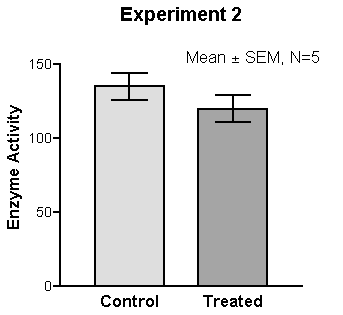
\includegraphics{images/error_bars} \end{center}

\section{Box plots}\label{box-plots}

 Box plots can convey more information about possible outcomes than a
range alone

\subsection{Box plots can help the audience understand the underlying
distribution of possible outcomes in more detail than just a range.
Typically they show the median, interquartile range, maximum and minimum
values for the range of possible outcomes. This can be particularly
useful when the underlying distribution is skewed or
non-normal.}\label{box-plots-can-help-the-audience-understand-the-underlying-distribution-of-possible-outcomes-in-more-detail-than-just-a-range.-typically-they-show-the-median-interquartile-range-maximum-and-minimum-values-for-the-range-of-possible-outcomes.-this-can-be-particularly-useful-when-the-underlying-distribution-is-skewed-or-non-normal.}

\subsection{Box plots can be arranged in parallel to show the
distributions for a range of measures, and can help compare the
different
shapes.}\label{box-plots-can-be-arranged-in-parallel-to-show-the-distributions-for-a-range-of-measures-and-can-help-compare-the-different-shapes.}

 A series of box plots can be used to compare distributions

\subsection{Box plots may not be widely understood by non-analysts, so
think carefully about whether the added information will be effective,
or whether a simple range would be sufficient. A labelled example can be
used to help the audience interpret the
format.}\label{box-plots-may-not-be-widely-understood-by-non-analysts-so-think-carefully-about-whether-the-added-information-will-be-effective-or-whether-a-simple-range-would-be-sufficient.-a-labelled-example-can-be-used-to-help-the-audience-interpret-the-format.}

 Think about whether the audience will be familiar with the format

\begin{Shaded}
\begin{Highlighting}[]
\NormalTok{knitr}\OperatorTok{::}\KeywordTok{include_graphics}\NormalTok{(}\StringTok{"images/box_plots.png"}\NormalTok{)}
\end{Highlighting}
\end{Shaded}

\begin{center}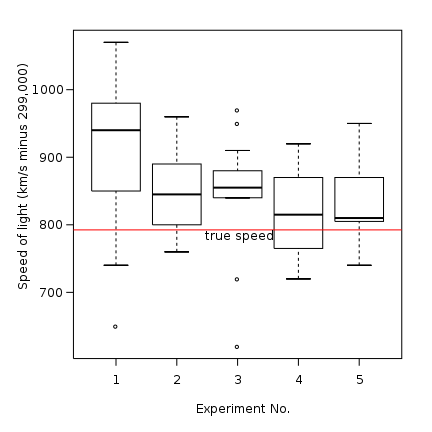
\includegraphics{images/box_plots} \end{center}

\section{Probability density functions
(PDFs)}\label{probability-density-functions-pdfs}

 PDFs show complete information on the quantified uncertainty

\subsection{A probability density function can be used to give complete
information on the range of possible outcomes, and the likelihood of
each for a given
estimate.}\label{a-probability-density-function-can-be-used-to-give-complete-information-on-the-range-of-possible-outcomes-and-the-likelihood-of-each-for-a-given-estimate.}

\subsection{While presenting complete information may seem ideal, it may
be more information than the audience actually needs. Would a prose
description of the mean and range be
sufficient?}\label{while-presenting-complete-information-may-seem-ideal-it-may-be-more-information-than-the-audience-actually-needs.-would-a-prose-description-of-the-mean-and-range-be-sufficient}

 Think about whether the audience needs this much information

\subsection{If the PDF is approximately normal, then there may be little
value in displaying it, as the essential features can be described in a
few
words.}\label{if-the-pdf-is-approximately-normal-then-there-may-be-little-value-in-displaying-it-as-the-essential-features-can-be-described-in-a-few-words.}

 PDFs can be useful when the distribution of outcomes is multimodal, or
otherwise complex

\subsection{However, if the distribution is multimodal , then it could
be misleading to present the mean, so a graphical illustration of the
distribution may be more
effective.}\label{however-if-the-distribution-is-multimodal-then-it-could-be-misleading-to-present-the-mean-so-a-graphical-illustration-of-the-distribution-may-be-more-effective.}

\subsection{It may aid clarity to draw the reader's attention to
important features, such as the
mode.}\label{it-may-aid-clarity-to-draw-the-readers-attention-to-important-features-such-as-the-mode.}

 Labelling can be used to highlight the key features

\begin{Shaded}
\begin{Highlighting}[]
\NormalTok{knitr}\OperatorTok{::}\KeywordTok{include_graphics}\NormalTok{(}\StringTok{"images/pdf.png"}\NormalTok{)}
\end{Highlighting}
\end{Shaded}

\begin{center}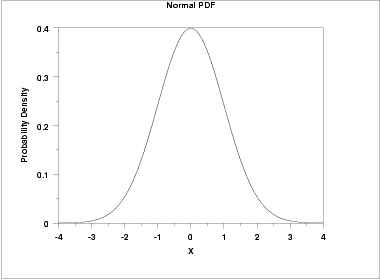
\includegraphics{images/pdf} \end{center}

\section{Multiple Probability Density
Functions}\label{multiple-probability-density-functions}

 Small multiples can be used to show the uncertainty across a number of
different measures

\subsection{If we need to communicate a series of PDFs, then multiple
functions can be shown to compare the range of possible outcomes across
the
series.}\label{if-we-need-to-communicate-a-series-of-pdfs-then-multiple-functions-can-be-shown-to-compare-the-range-of-possible-outcomes-across-the-series.}

\subsection{\texorpdfstring{If there are only 2 or 3 these can be
overlaid to make it easy to compare. With more, `small multiples' are
likely to be
clearer.}{If there are only 2 or 3 these can be overlaid to make it easy to compare. With more, small multiples are likely to be clearer.}}\label{if-there-are-only-2-or-3-these-can-be-overlaid-to-make-it-easy-to-compare.-with-more-small-multiples-are-likely-to-be-clearer.}

\begin{Shaded}
\begin{Highlighting}[]
\NormalTok{knitr}\OperatorTok{::}\KeywordTok{include_graphics}\NormalTok{(}\StringTok{"images/multiple_pdf.png"}\NormalTok{)}
\end{Highlighting}
\end{Shaded}

\begin{center}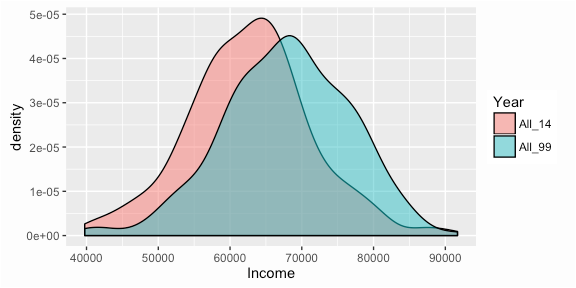
\includegraphics{images/multiple_pdf} \end{center}

\subsection{Violin plots are essentially mirrored PDFs which can be more
aesthetic. Additional information (such as box plots) can be overlaid if
required.}\label{violin-plots-are-essentially-mirrored-pdfs-which-can-be-more-aesthetic.-additional-information-such-as-box-plots-can-be-overlaid-if-required.}

 Violin plots can be used to compare PDFs

\begin{Shaded}
\begin{Highlighting}[]
\NormalTok{knitr}\OperatorTok{::}\KeywordTok{include_graphics}\NormalTok{(}\StringTok{"images/violin_plots.png"}\NormalTok{)}
\end{Highlighting}
\end{Shaded}

\begin{center}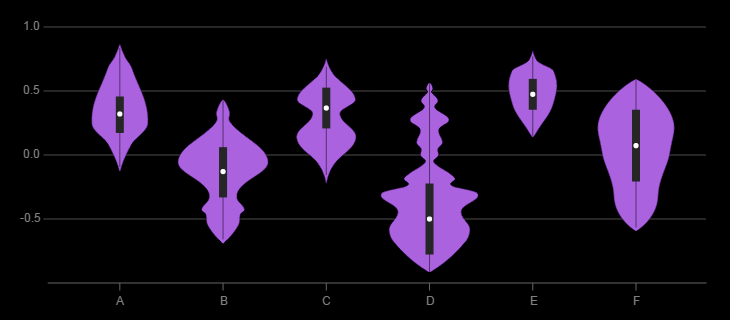
\includegraphics{images/violin_plots} \end{center}

\section{Cumulative density functions
(CDFs)}\label{cumulative-density-functions-cdfs}

 A CDF may be more helpful than a PDF if there is a specific threshold
of interest to the customer

\subsection{A cumulative density function essentially shows the same
information as a probability density function. However a CDF may be more
helpful when the audience is primarily concerned with how likely it is
that the value will be below (or above) a particular point (rather than
the range within which we expect the value to fall). For example , how
likely is it that our costs exceed our budget? (rather than what are our
costs going to
be?)}\label{a-cumulative-density-function-essentially-shows-the-same-information-as-a-probability-density-function.-however-a-cdf-may-be-more-helpful-when-the-audience-is-primarily-concerned-with-how-likely-it-is-that-the-value-will-be-below-or-above-a-particular-point-rather-than-the-range-within-which-we-expect-the-value-to-fall.-for-example-how-likely-is-it-that-our-costs-exceed-our-budget-rather-than-what-are-our-costs-going-to-be}

\subsection{However, features such as the mode are less clear on a CDF
(shown by the steepest part of the graph), as they are harder to read by
eye.}\label{however-features-such-as-the-mode-are-less-clear-on-a-cdf-shown-by-the-steepest-part-of-the-graph-as-they-are-harder-to-read-by-eye.}

 The most likely value is less clear on a CDF

\subsection{\texorpdfstring{Drawing gridlines intersecting at key points
of the function can help the viewer understand how to `read' the
graph.}{Drawing gridlines intersecting at key points of the function can help the viewer understand how to read the graph.}}\label{drawing-gridlines-intersecting-at-key-points-of-the-function-can-help-the-viewer-understand-how-to-read-the-graph.}

 Labelling can be used to highlight the key features

\begin{Shaded}
\begin{Highlighting}[]
\NormalTok{knitr}\OperatorTok{::}\KeywordTok{include_graphics}\NormalTok{(}\StringTok{"images/cdf.png"}\NormalTok{)}
\end{Highlighting}
\end{Shaded}

\begin{center}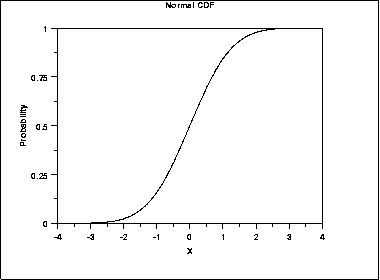
\includegraphics{images/cdf} \end{center}

\section{Fan Charts}\label{fan-charts}

 Fan charts can show how uncertainty changes over time

\subsection{Fan charts can be used to show a series of different
prediction intervals for time-series projections (e.g.~30\%, 60\% and
90\% at the same
time).}\label{fan-charts-can-be-used-to-show-a-series-of-different-prediction-intervals-for-time-series-projections-e.g.30-60-and-90-at-the-same-time.}

\subsection{This is essentially plotting selected points from a
time-dependent
PDF.}\label{this-is-essentially-plotting-selected-points-from-a-time-dependent-pdf.}

\subsection{\texorpdfstring{Often a central `best estimate' is not
included, to avoid the viewer focussing on a single estimate and
undermining the importance of the
uncertainty}{Often a central best estimate is not included, to avoid the viewer focussing on a single estimate and undermining the importance of the uncertainty}}\label{often-a-central-best-estimate-is-not-included-to-avoid-the-viewer-focussing-on-a-single-estimate-and-undermining-the-importance-of-the-uncertainty}

 Avoid including the mode

\begin{Shaded}
\begin{Highlighting}[]
\NormalTok{knitr}\OperatorTok{::}\KeywordTok{include_graphics}\NormalTok{(}\StringTok{"images/fan_chart.png"}\NormalTok{)}
\end{Highlighting}
\end{Shaded}

\begin{center}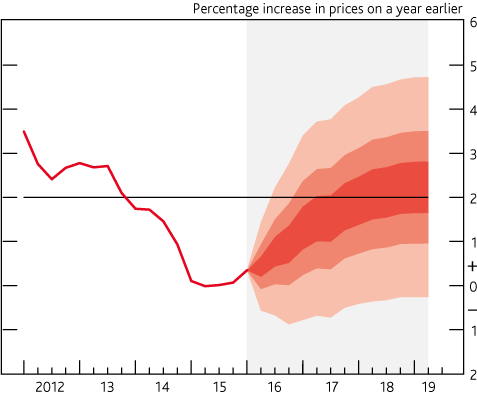
\includegraphics{images/fan_chart} \end{center}

\section{Spaghetti Plots}\label{spaghetti-plots}

 Spaghetti plots can be used to show the results from a range of
different methodologies

\subsection{If the methodology is believed to be the dominant source of
uncertainty, then showing results with multiple different methodologies
can be
effective.}\label{if-the-methodology-is-believed-to-be-the-dominant-source-of-uncertainty-then-showing-results-with-multiple-different-methodologies-can-be-effective.}

\subsection{Less importance is placed on quantified uncertainties, and
more on the general consensus of
results.}\label{less-importance-is-placed-on-quantified-uncertainties-and-more-on-the-general-consensus-of-results.}

\subsection{Potential flaws are that all methodologies are given equal
weight, which may not be
appropriate.}\label{potential-flaws-are-that-all-methodologies-are-given-equal-weight-which-may-not-be-appropriate.}

 Other sources of uncertainty should be considered

\subsection{Also, the uncertainty within each methodology is not
shown.}\label{also-the-uncertainty-within-each-methodology-is-not-shown.}

\begin{Shaded}
\begin{Highlighting}[]
\NormalTok{knitr}\OperatorTok{::}\KeywordTok{include_graphics}\NormalTok{(}\StringTok{"images/spaghetti.png"}\NormalTok{)}
\end{Highlighting}
\end{Shaded}

\begin{center}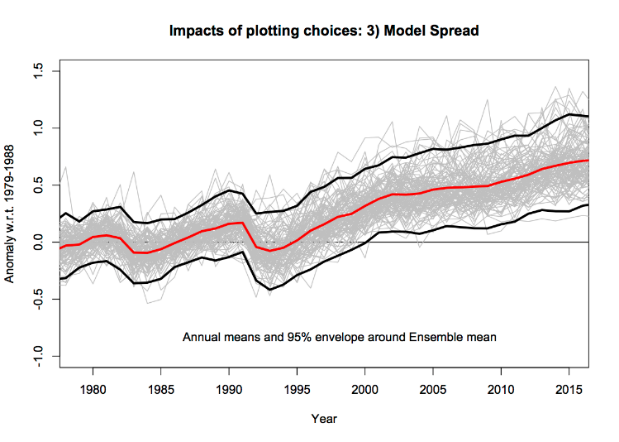
\includegraphics{images/spaghetti} \end{center}

\section{Multiple Line Charts}\label{multiple-line-charts}

Multiple line charts can be clearer than a series of error bars

\subsection{\texorpdfstring{Multiple line charts with time series data
to show a quantified range around a `most likely' projection
(essentially a series of error
bars).}{Multiple line charts with time series data to show a quantified range around a most likely projection (essentially a series of error bars).}}\label{multiple-line-charts-with-time-series-data-to-show-a-quantified-range-around-a-most-likely-projection-essentially-a-series-of-error-bars.}

\subsection{With scenario analysis, a series of line charts can be used
to show the projections from each
scenario.}\label{with-scenario-analysis-a-series-of-line-charts-can-be-used-to-show-the-projections-from-each-scenario.}

Alternative scenarios can be illustrated with multiple line graphs

\subsection{Generally with scenario analysis each scenario should be
presented with equal prominence, to avoid suggesting that one is more
likely than another (unless analysis has been carried out to quantify
the likelihoods of
each).}\label{generally-with-scenario-analysis-each-scenario-should-be-presented-with-equal-prominence-to-avoid-suggesting-that-one-is-more-likely-than-another-unless-analysis-has-been-carried-out-to-quantify-the-likelihoods-of-each.}

Give equal prominence to each scenario

\subsection{\texorpdfstring{Try to include an even number of scenarios,
to avoid having a middle option that may be misinterpreted as the `most
likely'
scenario.}{Try to include an even number of scenarios, to avoid having a middle option that may be misinterpreted as the most likely scenario.}}\label{try-to-include-an-even-number-of-scenarios-to-avoid-having-a-middle-option-that-may-be-misinterpreted-as-the-most-likely-scenario.}

 Try to have an even number of scenarios

\begin{Shaded}
\begin{Highlighting}[]
\NormalTok{knitr}\OperatorTok{::}\KeywordTok{include_graphics}\NormalTok{(}\StringTok{"images/multiple+line.png"}\NormalTok{)}
\end{Highlighting}
\end{Shaded}

\begin{center}\includegraphics{images/multiple+line} \end{center}

\section{Tornado Diagrams}\label{tornado-diagrams}

Tornado diagrams can be used to show the sources of uncertainty

\subsection{Tornado diagrams are different to most other graphs
discussed here. They are not used to show the outputs of the analysis,
but to show how different sources of uncertainty contribute to the
overall
uncertainty.}\label{tornado-diagrams-are-different-to-most-other-graphs-discussed-here.-they-are-not-used-to-show-the-outputs-of-the-analysis-but-to-show-how-different-sources-of-uncertainty-contribute-to-the-overall-uncertainty.}

\subsection{Tornado diagrams depict sensitivity of a result to changes
in selected
variables.}\label{tornado-diagrams-depict-sensitivity-of-a-result-to-changes-in-selected-variables.}

\subsection{They show the effect on the output of varying each variable
at a time, keeping other input variables at their assumed
values.}\label{they-show-the-effect-on-the-output-of-varying-each-variable-at-a-time-keeping-other-input-variables-at-their-assumed-values.}

\subsection{If the level of uncertainty is unpalatable to the customers,
then this format can be useful to help focus work on reducing the level
of uncertainty in key
parameters.}\label{if-the-level-of-uncertainty-is-unpalatable-to-the-customers-then-this-format-can-be-useful-to-help-focus-work-on-reducing-the-level-of-uncertainty-in-key-parameters.}

 Can help communicate the reasons for uncertainty, and identify further
need for analysis

\subsection{One limitation of the format is that only one parameter is
changed at a time. There are some situations where the uncertainty due
to one variable may appear small initially, but becomes much more
prominent if a second variable takes on a slightly different value
(e.g.~think of a workflow model with a bottleneck. A tornado diagram
might show the bottleneck parameter to be the overwhelming uncertainty.
However, if this parameter is increased slightly then the bottleneck may
move elsewhere, completely changing the
picture)}\label{one-limitation-of-the-format-is-that-only-one-parameter-is-changed-at-a-time.-there-are-some-situations-where-the-uncertainty-due-to-one-variable-may-appear-small-initially-but-becomes-much-more-prominent-if-a-second-variable-takes-on-a-slightly-different-value-e.g.think-of-a-workflow-model-with-a-bottleneck.-a-tornado-diagram-might-show-the-bottleneck-parameter-to-be-the-overwhelming-uncertainty.-however-if-this-parameter-is-increased-slightly-then-the-bottleneck-may-move-elsewhere-completely-changing-the-picture}

 Tornado diagrams can be misleading in complex models

\begin{Shaded}
\begin{Highlighting}[]
\NormalTok{knitr}\OperatorTok{::}\KeywordTok{include_graphics}\NormalTok{(}\StringTok{"images/tornado.png"}\NormalTok{)}
\end{Highlighting}
\end{Shaded}

\begin{center}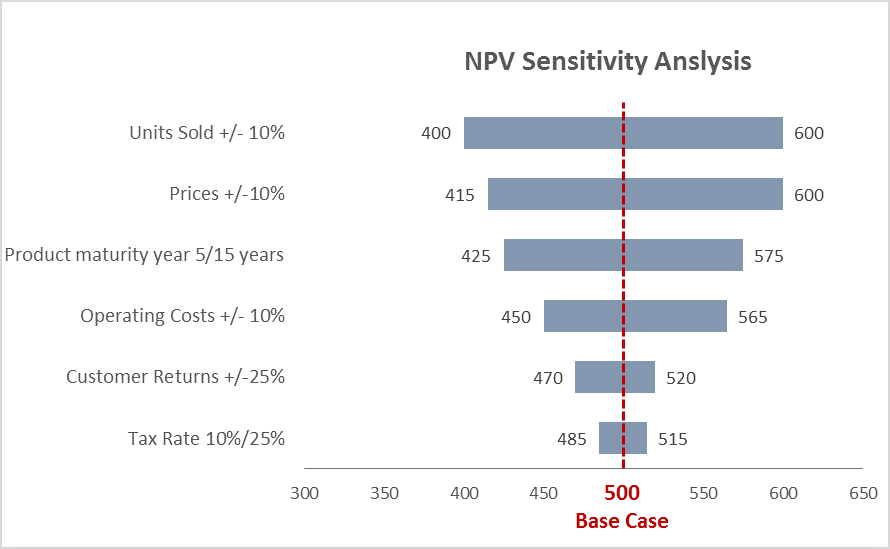
\includegraphics{images/tornado} \end{center}

\section{Infographics}\label{infographics}

 Infographics can be useful for public facing communications

\subsection{Infographics are graphic visual representations of
information, data or knowledge intended to present information quickly
and clearly. They can improve people's understanding by using graphics
to enhance peoples' ability to see patterns and
trends.}\label{infographics-are-graphic-visual-representations-of-information-data-or-knowledge-intended-to-present-information-quickly-and-clearly.-they-can-improve-peoples-understanding-by-using-graphics-to-enhance-peoples-ability-to-see-patterns-and-trends.}

\subsection{When done well they will grab the reader's attention from
their otherwise busy day and become a very powerful way of communicating
key
messages.}\label{when-done-well-they-will-grab-the-readers-attention-from-their-otherwise-busy-day-and-become-a-very-powerful-way-of-communicating-key-messages.}

 They grab attention

\subsection{Investing in and designing a good infographic may be
worthwhile if your audience is less confident with data and
analysis.}\label{investing-in-and-designing-a-good-infographic-may-be-worthwhile-if-your-audience-is-less-confident-with-data-and-analysis.}

 The additional graphics and text make your charts and messages more
accessible

\subsection{An example where uncertainty in the form of confidence
intervals has been explained using an infographic is in the Households
Below Average Income Report, ONS
:}\label{an-example-where-uncertainty-in-the-form-of-confidence-intervals-has-been-explained-using-an-infographic-is-in-the-households-below-average-income-report-ons}

 Example -- confidence intervals

\begin{Shaded}
\begin{Highlighting}[]
\NormalTok{knitr}\OperatorTok{::}\KeywordTok{include_graphics}\NormalTok{(}\StringTok{"images/infographic.png"}\NormalTok{)}
\end{Highlighting}
\end{Shaded}

\begin{center}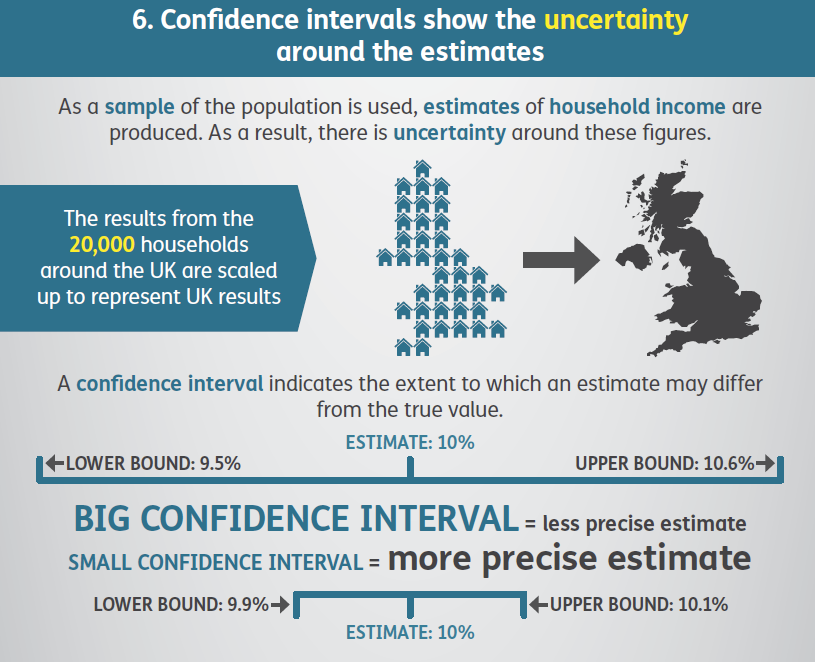
\includegraphics{images/infographic} \end{center}

\subsection{A simple infographic can be used to help the reader
visualise the relative magnitude of numbers. This may be useful if we
want to demonstrate either the magnitude of the uncertainty relative to
the overall result. E.g. below helps the reader to interpret four
percentages10}\label{a-simple-infographic-can-be-used-to-help-the-reader-visualise-the-relative-magnitude-of-numbers.-this-may-be-useful-if-we-want-to-demonstrate-either-the-magnitude-of-the-uncertainty-relative-to-the-overall-result.-e.g.-below-helps-the-reader-to-interpret-four-percentages10}

 Visualise relative magnitudes

\begin{Shaded}
\begin{Highlighting}[]
\NormalTok{knitr}\OperatorTok{::}\KeywordTok{include_graphics}\NormalTok{(}\StringTok{"images/infographic.png"}\NormalTok{)}
\end{Highlighting}
\end{Shaded}

\begin{center}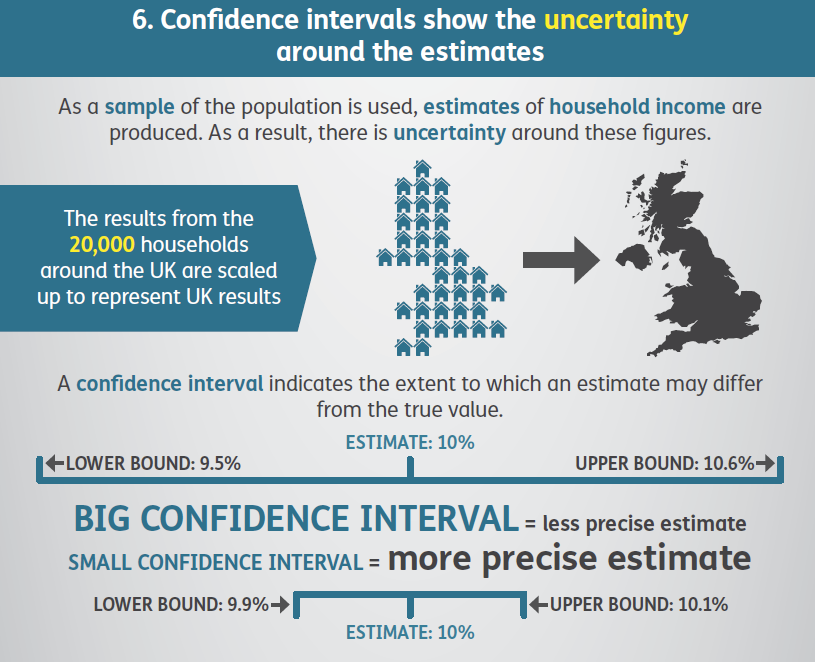
\includegraphics{images/infographic} \end{center}

\subsection{Infographics can use a lot of space and can become overly
simplistic. Consider the format being used to determine if an
infographic is the right
choice.}\label{infographics-can-use-a-lot-of-space-and-can-become-overly-simplistic.-consider-the-format-being-used-to-determine-if-an-infographic-is-the-right-choice.}

 Avoid common pitfalls

\subsection{\texorpdfstring{For wider principles of good infographic
design and common mistakes to avoid see:
\url{https://www.nngroup.com/articles/designing-effective-infographics/}}{For wider principles of good infographic design and common mistakes to avoid see: https://www.nngroup.com/articles/designing-effective-infographics/}}\label{for-wider-principles-of-good-infographic-design-and-common-mistakes-to-avoid-see-httpswww.nngroup.comarticlesdesigning-effective-infographics}

 Refer to other sources for general principles around infographic design

\section{Interactive Tools}\label{interactive-tools}

 Interactive tools can be used to immerse your reader on complex matters

\subsection{An interactive tool can help to bring analysis to life and
make it more accessible to non-specialists. They can create an immersive
experience that is easier for them to understand and is highly
memorable.}\label{an-interactive-tool-can-help-to-bring-analysis-to-life-and-make-it-more-accessible-to-non-specialists.-they-can-create-an-immersive-experience-that-is-easier-for-them-to-understand-and-is-highly-memorable.}

\subsection{Consider the overall message and where the uncertainties
lie. Which aspects will the audience be interested in and what do they
need to hear? Use this understanding to bring focus to which interactive
elements to
create.}\label{consider-the-overall-message-and-where-the-uncertainties-lie.-which-aspects-will-the-audience-be-interested-in-and-what-do-they-need-to-hear-use-this-understanding-to-bring-focus-to-which-interactive-elements-to-create.}

 Focus on specific messages

\subsection{The interactivity will enable your users to manipulate and
get a deeper understanding of the
message.}\label{the-interactivity-will-enable-your-users-to-manipulate-and-get-a-deeper-understanding-of-the-message.}

\subsection{If a key source of uncertainty is a single variable, then it
may be possible to construct a display that can be changed as the user
adjusts the value of this variable by moving a
slider.}\label{if-a-key-source-of-uncertainty-is-a-single-variable-then-it-may-be-possible-to-construct-a-display-that-can-be-changed-as-the-user-adjusts-the-value-of-this-variable-by-moving-a-slider.}

 Allow reader to adjust a key variable

\subsection{Or, if there are several key assumptions that impact the
result a chart may be created that will change depending on the inputs
that the user
inserts.}\label{or-if-there-are-several-key-assumptions-that-impact-the-result-a-chart-may-be-created-that-will-change-depending-on-the-inputs-that-the-user-inserts.}

\subsection{Being able to see what would happen if an underlying
assumption was to change is a powerful way to demonstrate the level of
uncertainty we may have in a given
result.}\label{being-able-to-see-what-would-happen-if-an-underlying-assumption-was-to-change-is-a-powerful-way-to-demonstrate-the-level-of-uncertainty-we-may-have-in-a-given-result.}

\subsection{If the communication with the decision maker is limited to a
printed report, then interactive tools will not be
possible.}\label{if-the-communication-with-the-decision-maker-is-limited-to-a-printed-report-then-interactive-tools-will-not-be-possible.}

 Not possible on traditional printed format. Example - DECC 2050
Calculator

\subsection{\texorpdfstring{The
\href{http://2050-calculator-tool.decc.gov.uk/\#/calculator}{DECC 2050
Calculator} is an award-winning, user-friendly tool that helps users to
explore the choices available to meet the 2050 carbon target. Whilst it
doesn't explicitly cover the uncertainty in the underlying data it does
allow the user to create their own set of policies to try to reach the
target. This engaging tool was helpful in demonstrating to users how
difficult some of the options are and the relative impact of each
choice.}{The DECC 2050 Calculator is an award-winning, user-friendly tool that helps users to explore the choices available to meet the 2050 carbon target. Whilst it doesn't explicitly cover the uncertainty in the underlying data it does allow the user to create their own set of policies to try to reach the target. This engaging tool was helpful in demonstrating to users how difficult some of the options are and the relative impact of each choice.}}\label{the-decc-2050-calculator-is-an-award-winning-user-friendly-tool-that-helps-users-to-explore-the-choices-available-to-meet-the-2050-carbon-target.-whilst-it-doesnt-explicitly-cover-the-uncertainty-in-the-underlying-data-it-does-allow-the-user-to-create-their-own-set-of-policies-to-try-to-reach-the-target.-this-engaging-tool-was-helpful-in-demonstrating-to-users-how-difficult-some-of-the-options-are-and-the-relative-impact-of-each-choice.}

\bibliography{book.bib,packages.bib}


\end{document}
